\section{Registration}

{
\setbeamertemplate{background}{}
\setbeamertemplate{navigation symbols}{}
\setbeamercolor{background canvas}{bg={black}}
\color{white}
\begin{frame}[plain]
\fontsize{36pt}{36pt}\selectfont
\center
\begin{center}
Refactored Registration Framework
\end{center}

\fontsize{12pt}{12pt}\selectfont
\begin{center}
Insight Software Consortium
\end{center}
\vskip12pt
\begin{center}
 PICSL @ University of Pennsylvania 
\end{center}
\vskip12pt
\begin{center}
 Brian Avants, Nicholas Tustison, Gang Song, \\ 
Baohua Wu, Michael Stauffer, James C. Gee
\end{center}
\end{frame}
}

\subsection{Introduction}

\begin{frame}
\frametitle{What is registration?}
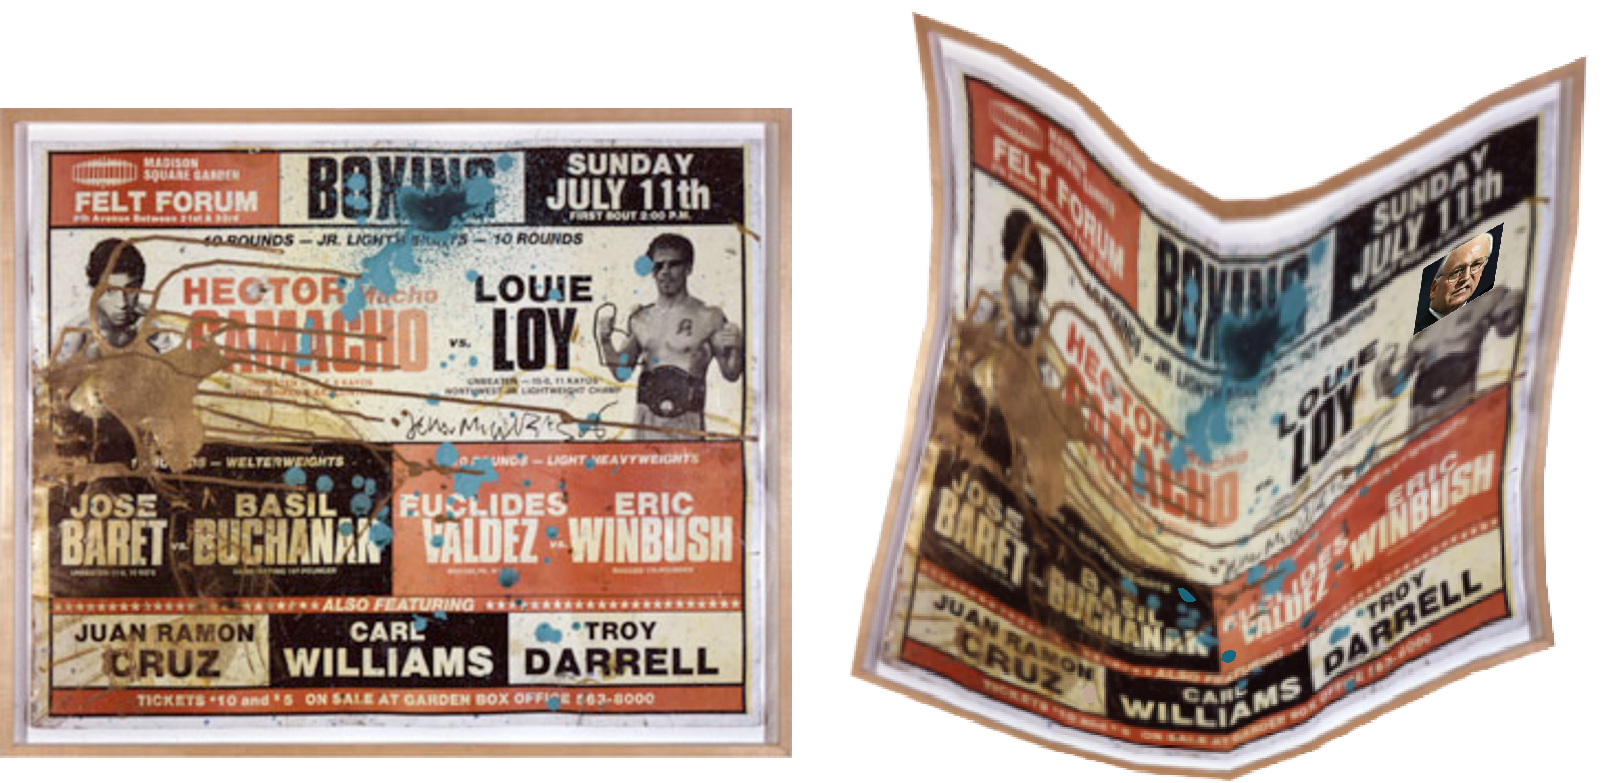
\includegraphics[height=2in]{../Art/RegistrationBasquiatWarp.pdf}
\end{frame}

\begin{frame}
\frametitle{What is registration?}
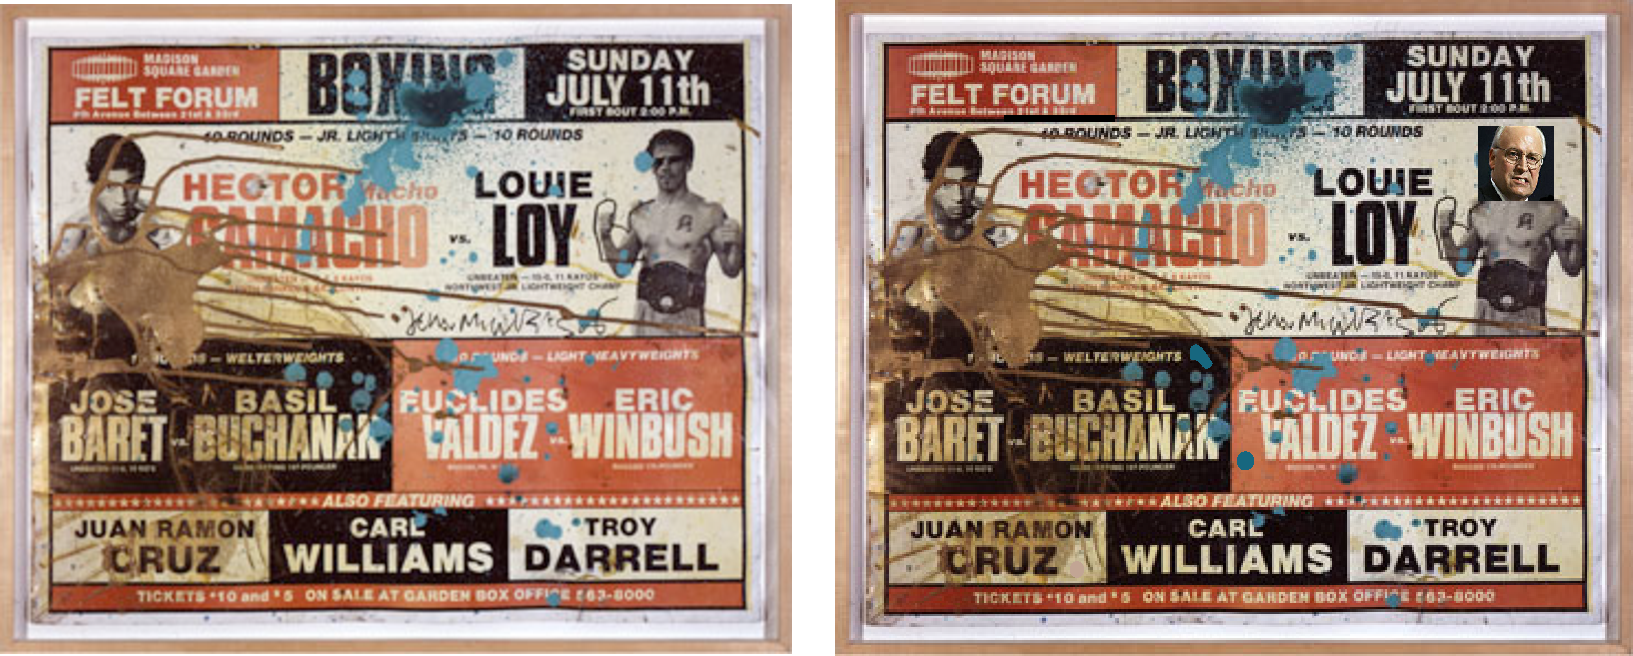
\includegraphics[height=1.8in]{../Art/RegistrationBasquiatDeWarp.pdf}
\vskip20pt
\begin{displaymath}
\| I ( x ) - J(\phi(x)) \|^2  + R(\phi( x))
\end{displaymath}
\end{frame}

\subsection{ITK Registration Framework}

\subsubsection{Image Resampling}

\begin{frame}
  \frametitle{Image Origin and Spacing}
  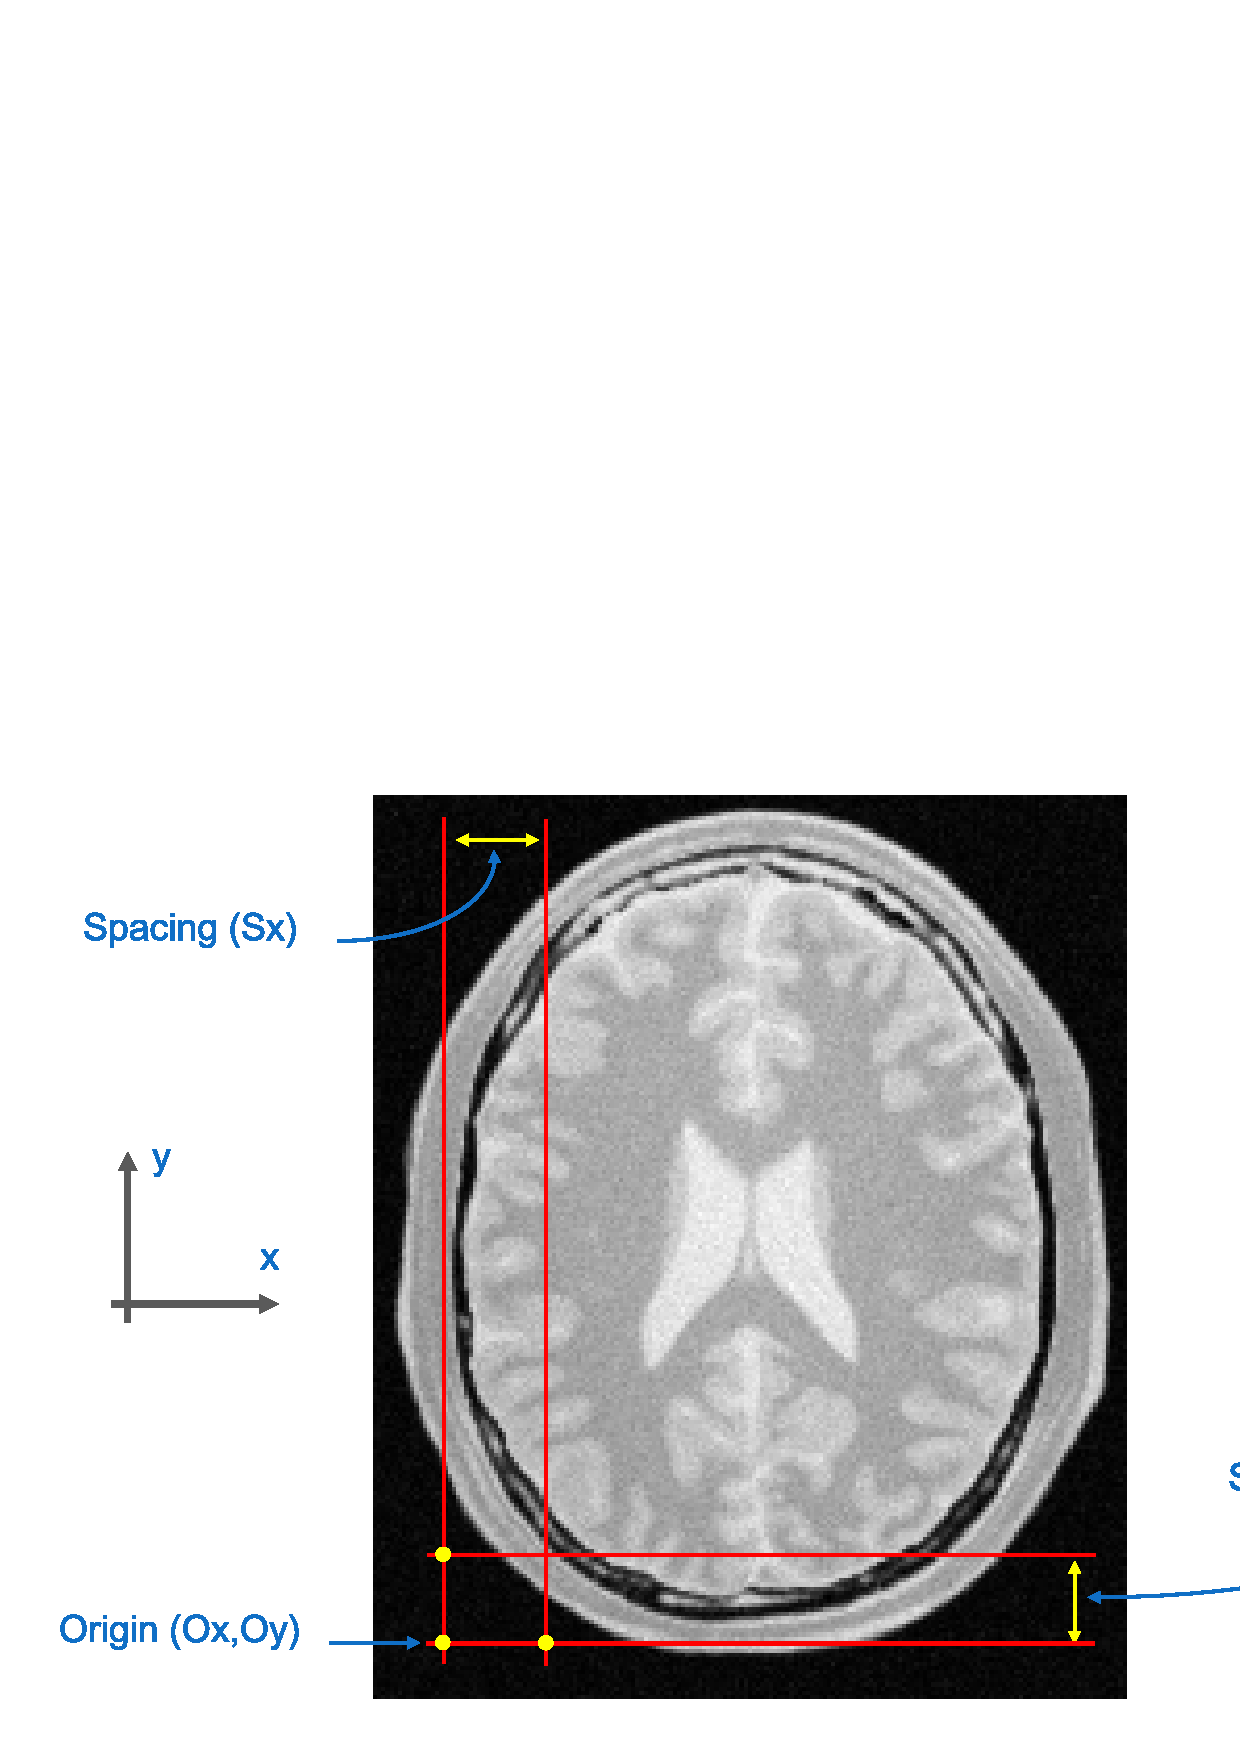
\includegraphics[width=0.8\textwidth]{../Art/Resampling01ImageOriginAndSpacing.pdf}
\end{frame}

\begin{frame}
  \frametitle{Image Sampling Grid}
  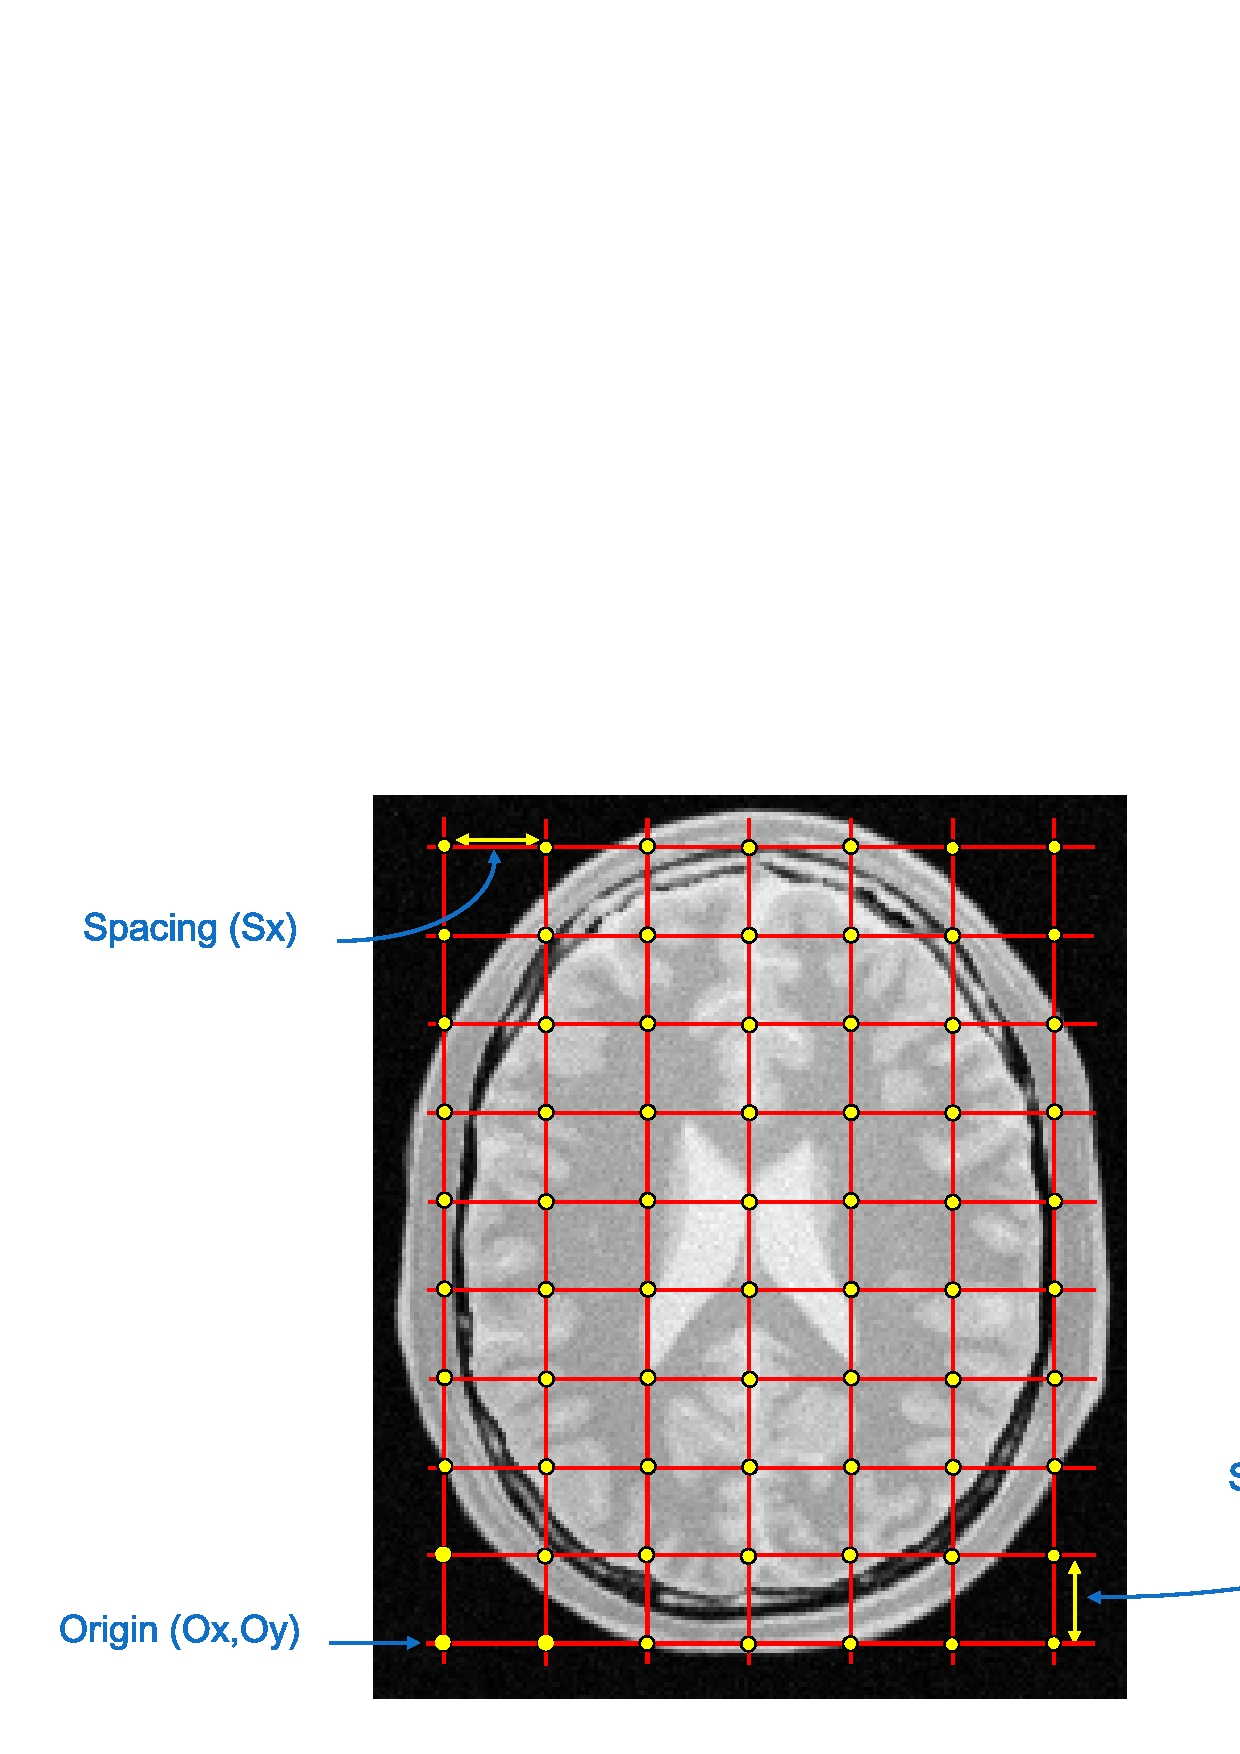
\includegraphics[width=0.8\textwidth]{../Art/Resampling02ImageSamplingGrid.pdf}
\end{frame}

\begin{frame}
  \frametitle{Image Pixel}
  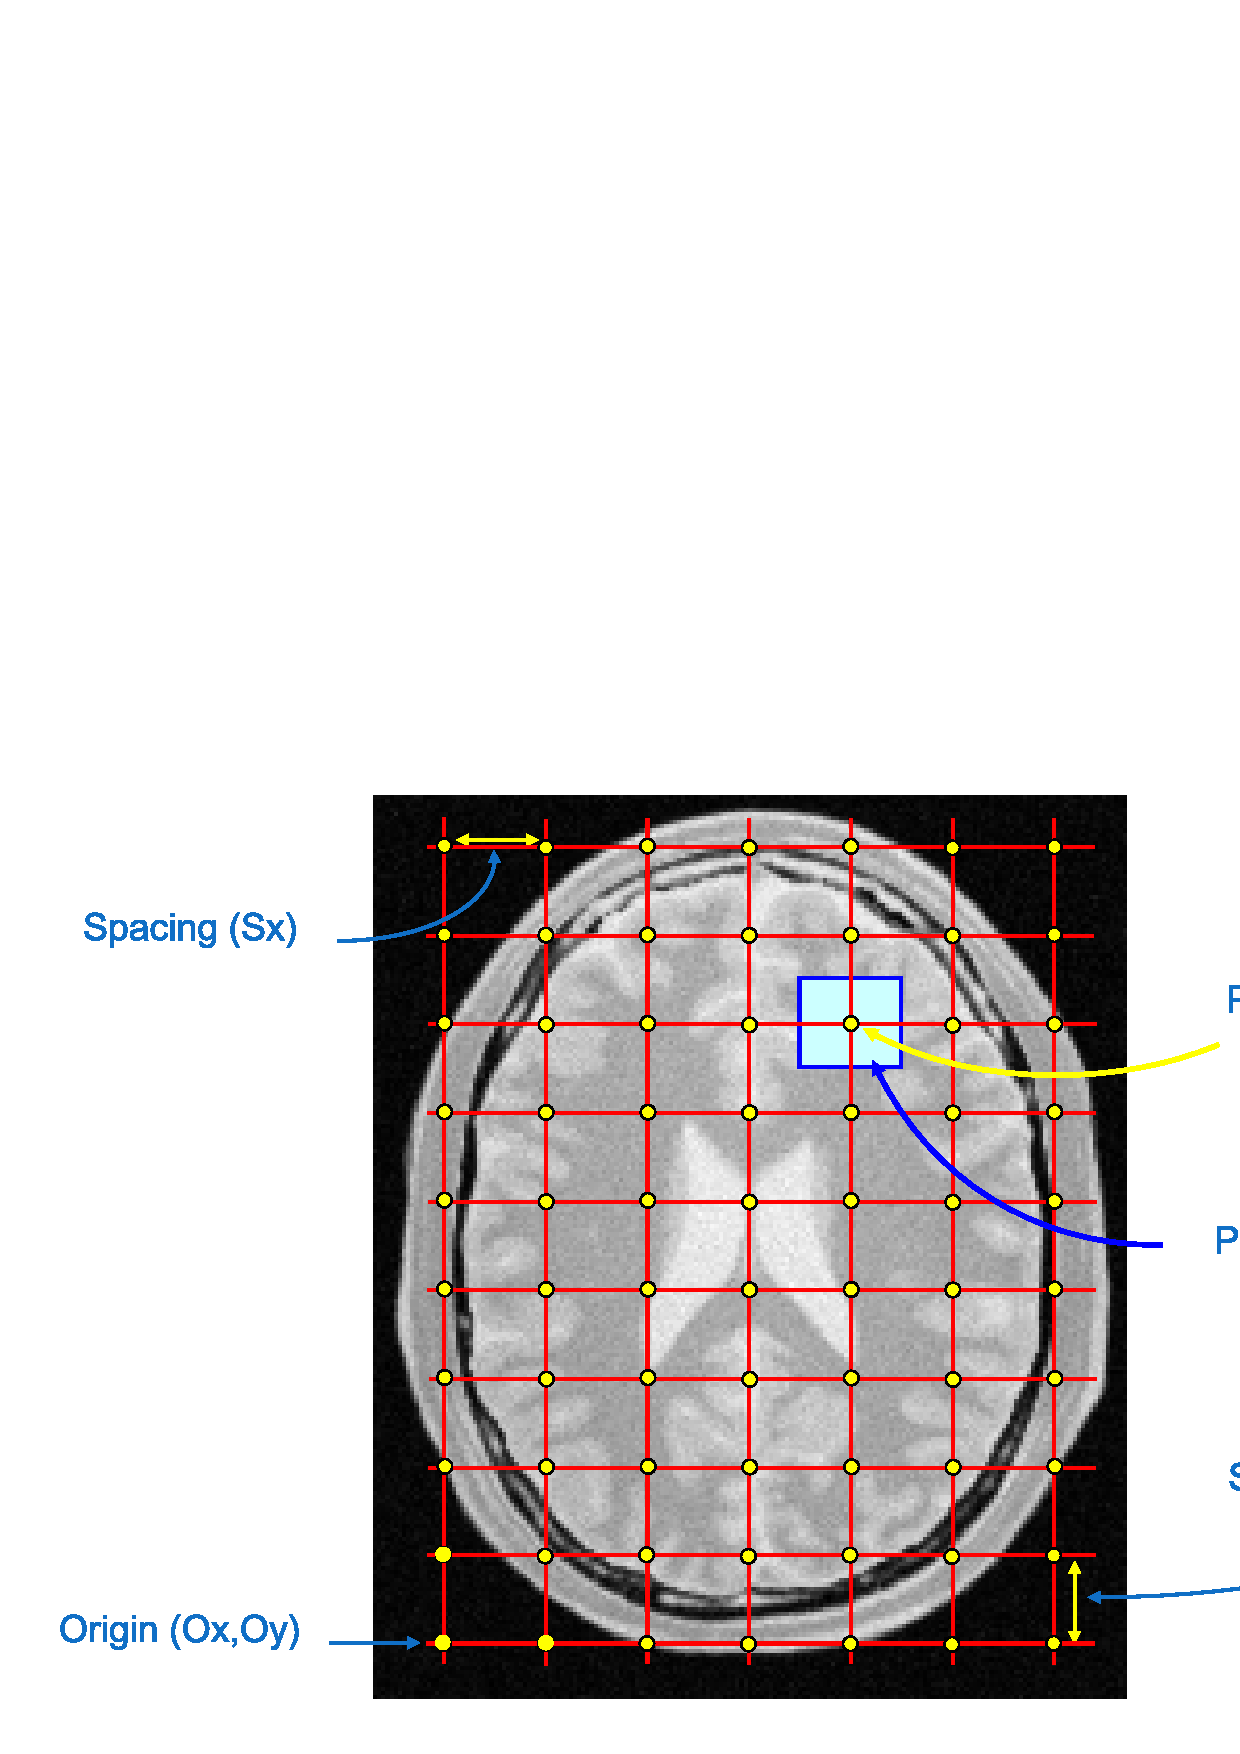
\includegraphics[width=0.8\textwidth]{../Art/Resampling03ImagePixel.pdf}
\end{frame}

\begin{frame}
  \frametitle{Image Indices}
  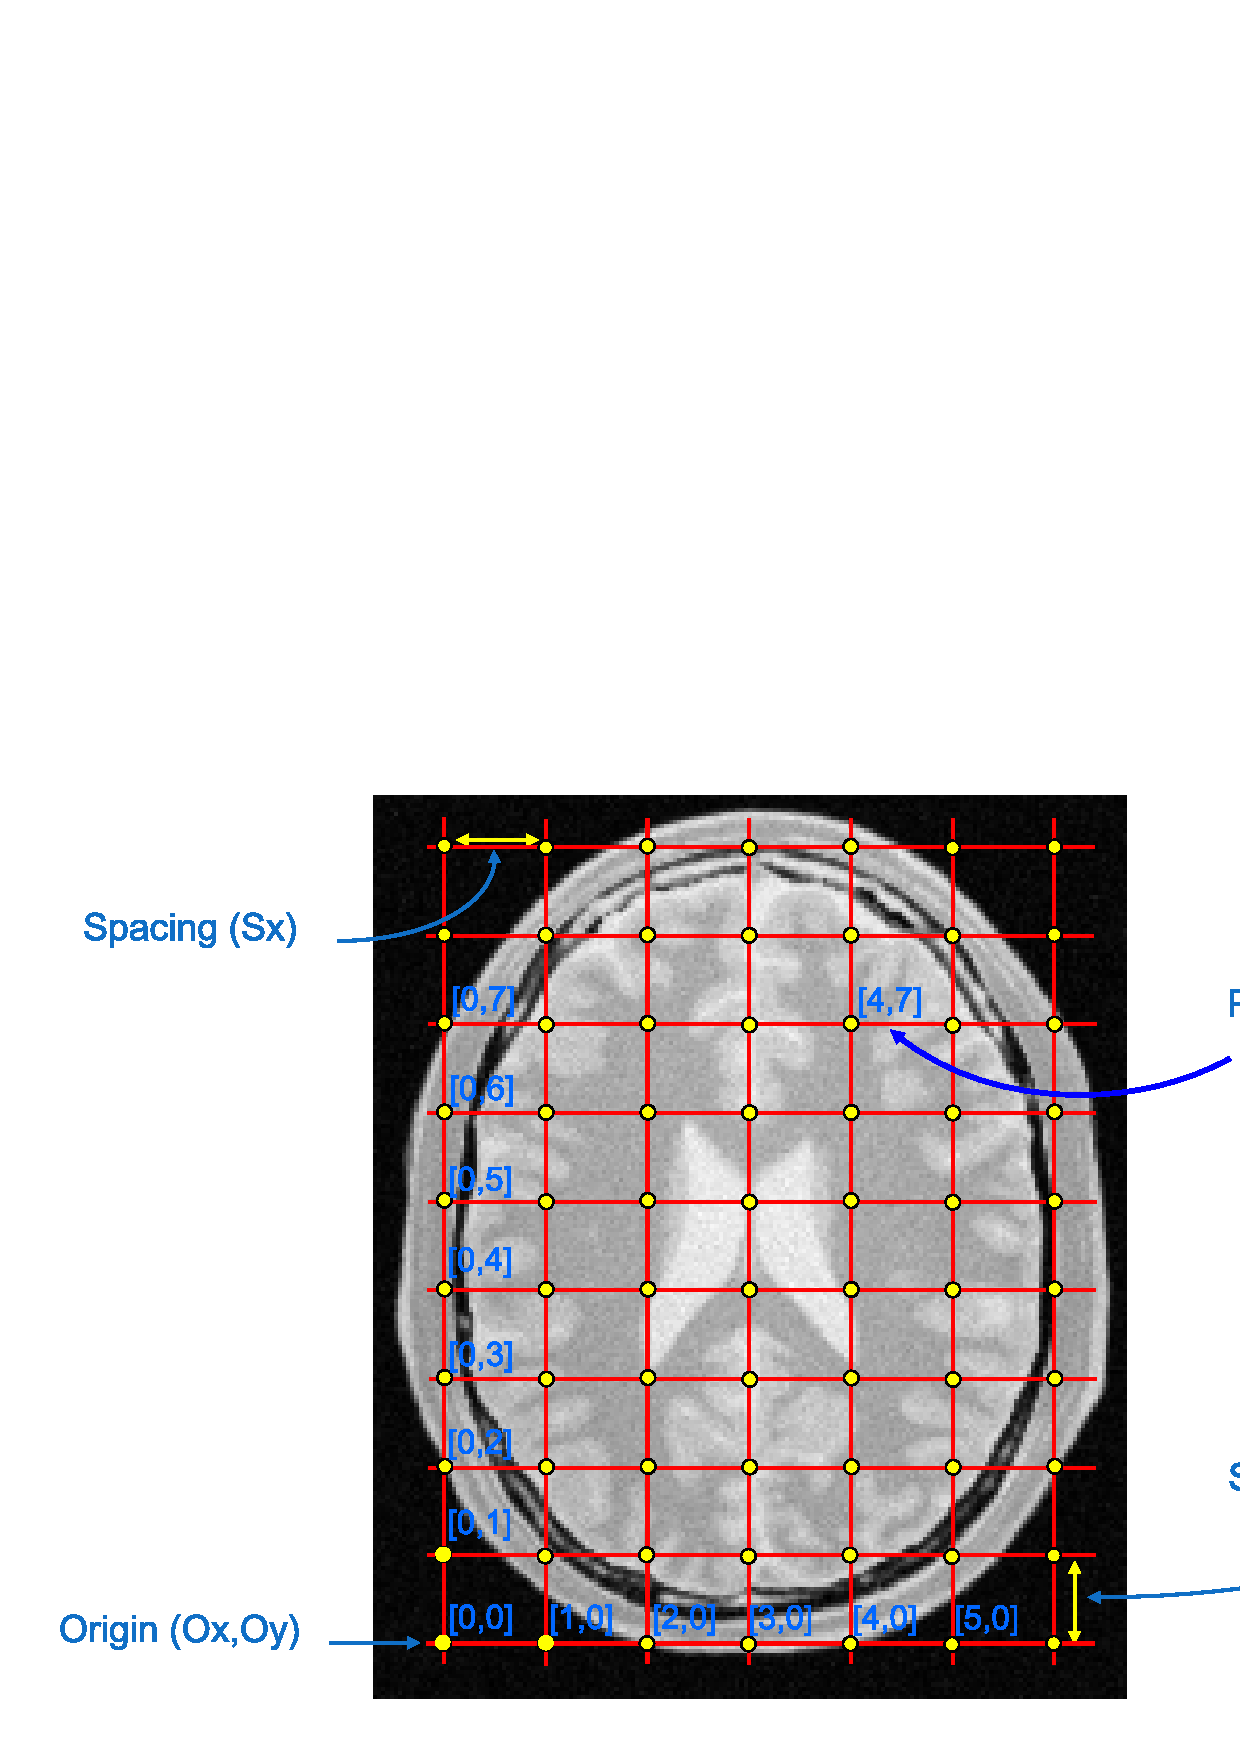
\includegraphics[width=0.8\textwidth]{../Art/Resampling04ImageIndices.pdf}
\end{frame}

\begin{frame}
  \frametitle{Image To Physical Coordinates}
  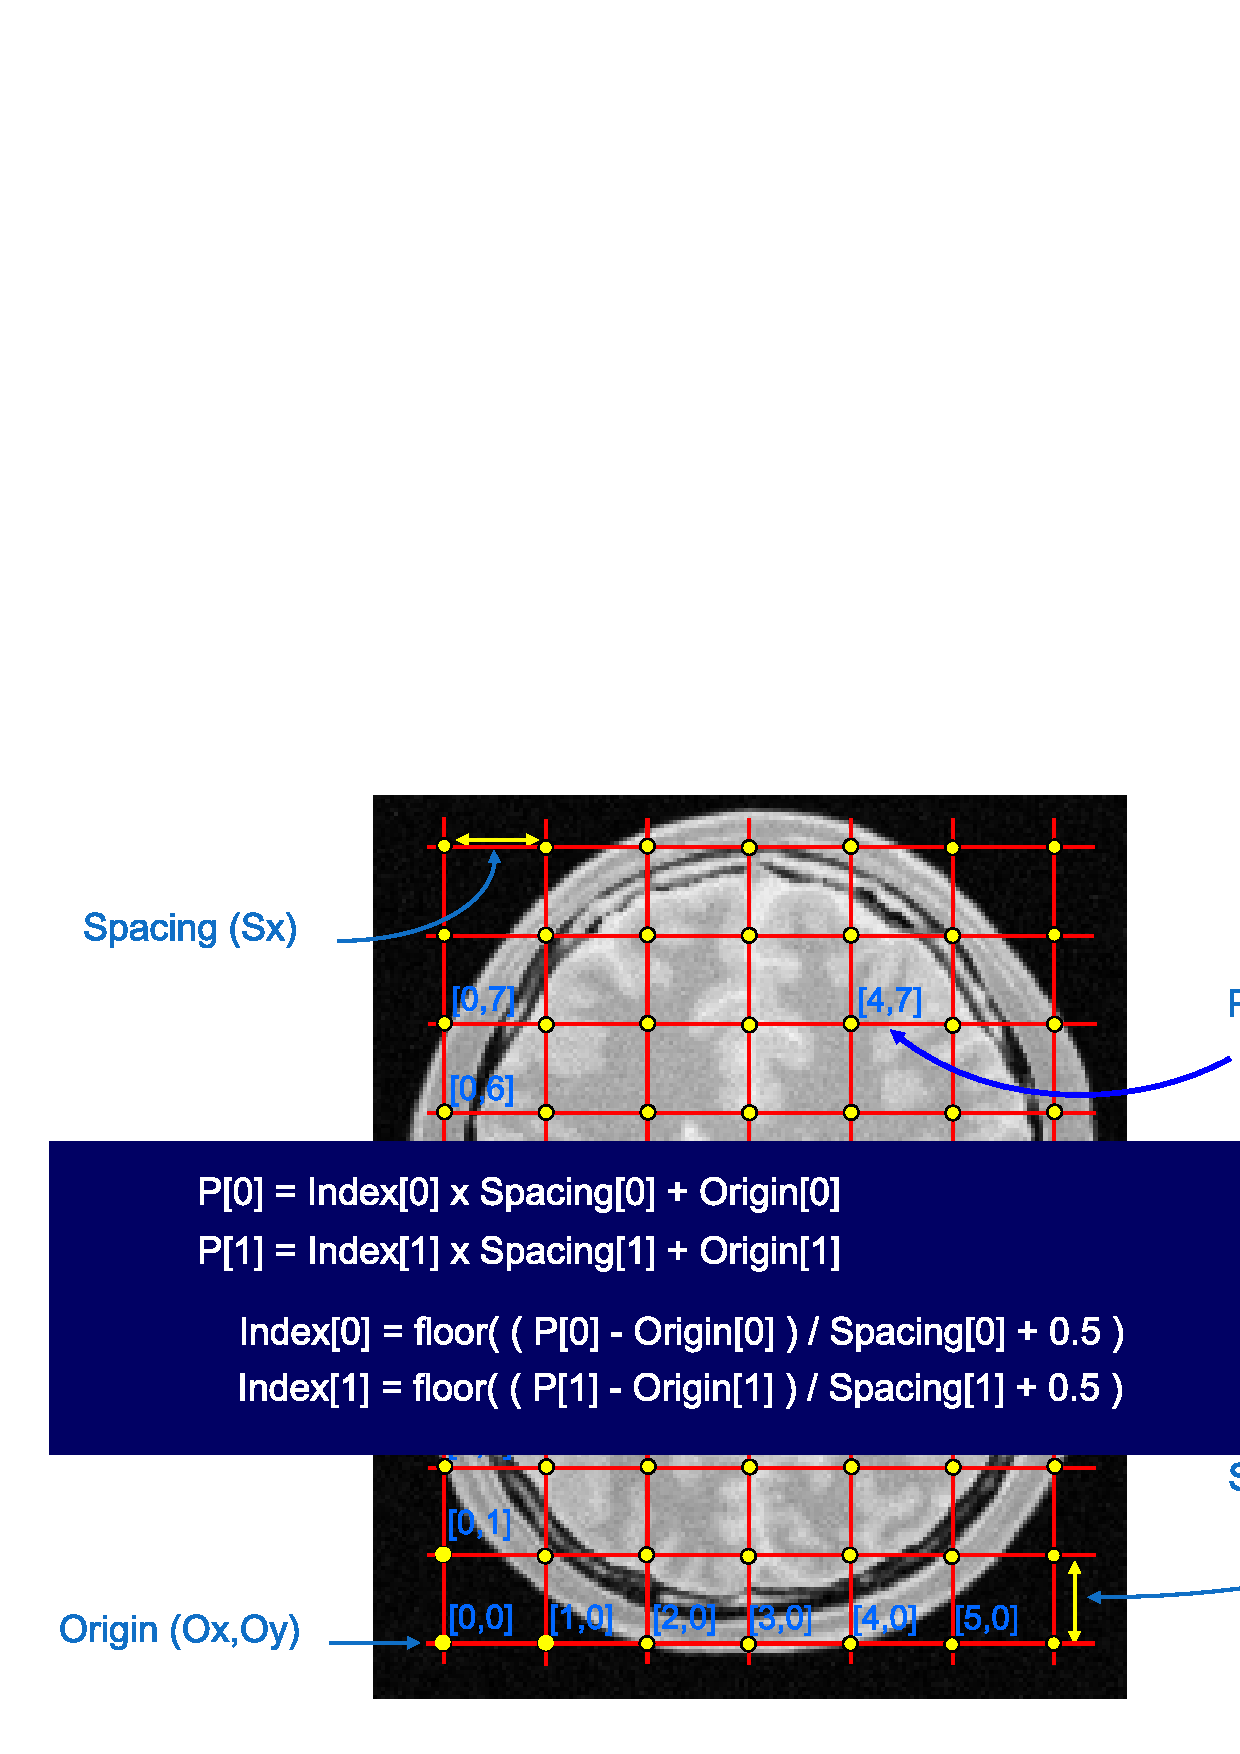
\includegraphics[width=0.8\textwidth]{../Art/Resampling05ImageToPhysicalCoordinates.pdf}
\end{frame}

\begin{frame}
  \frametitle{Image Region}
  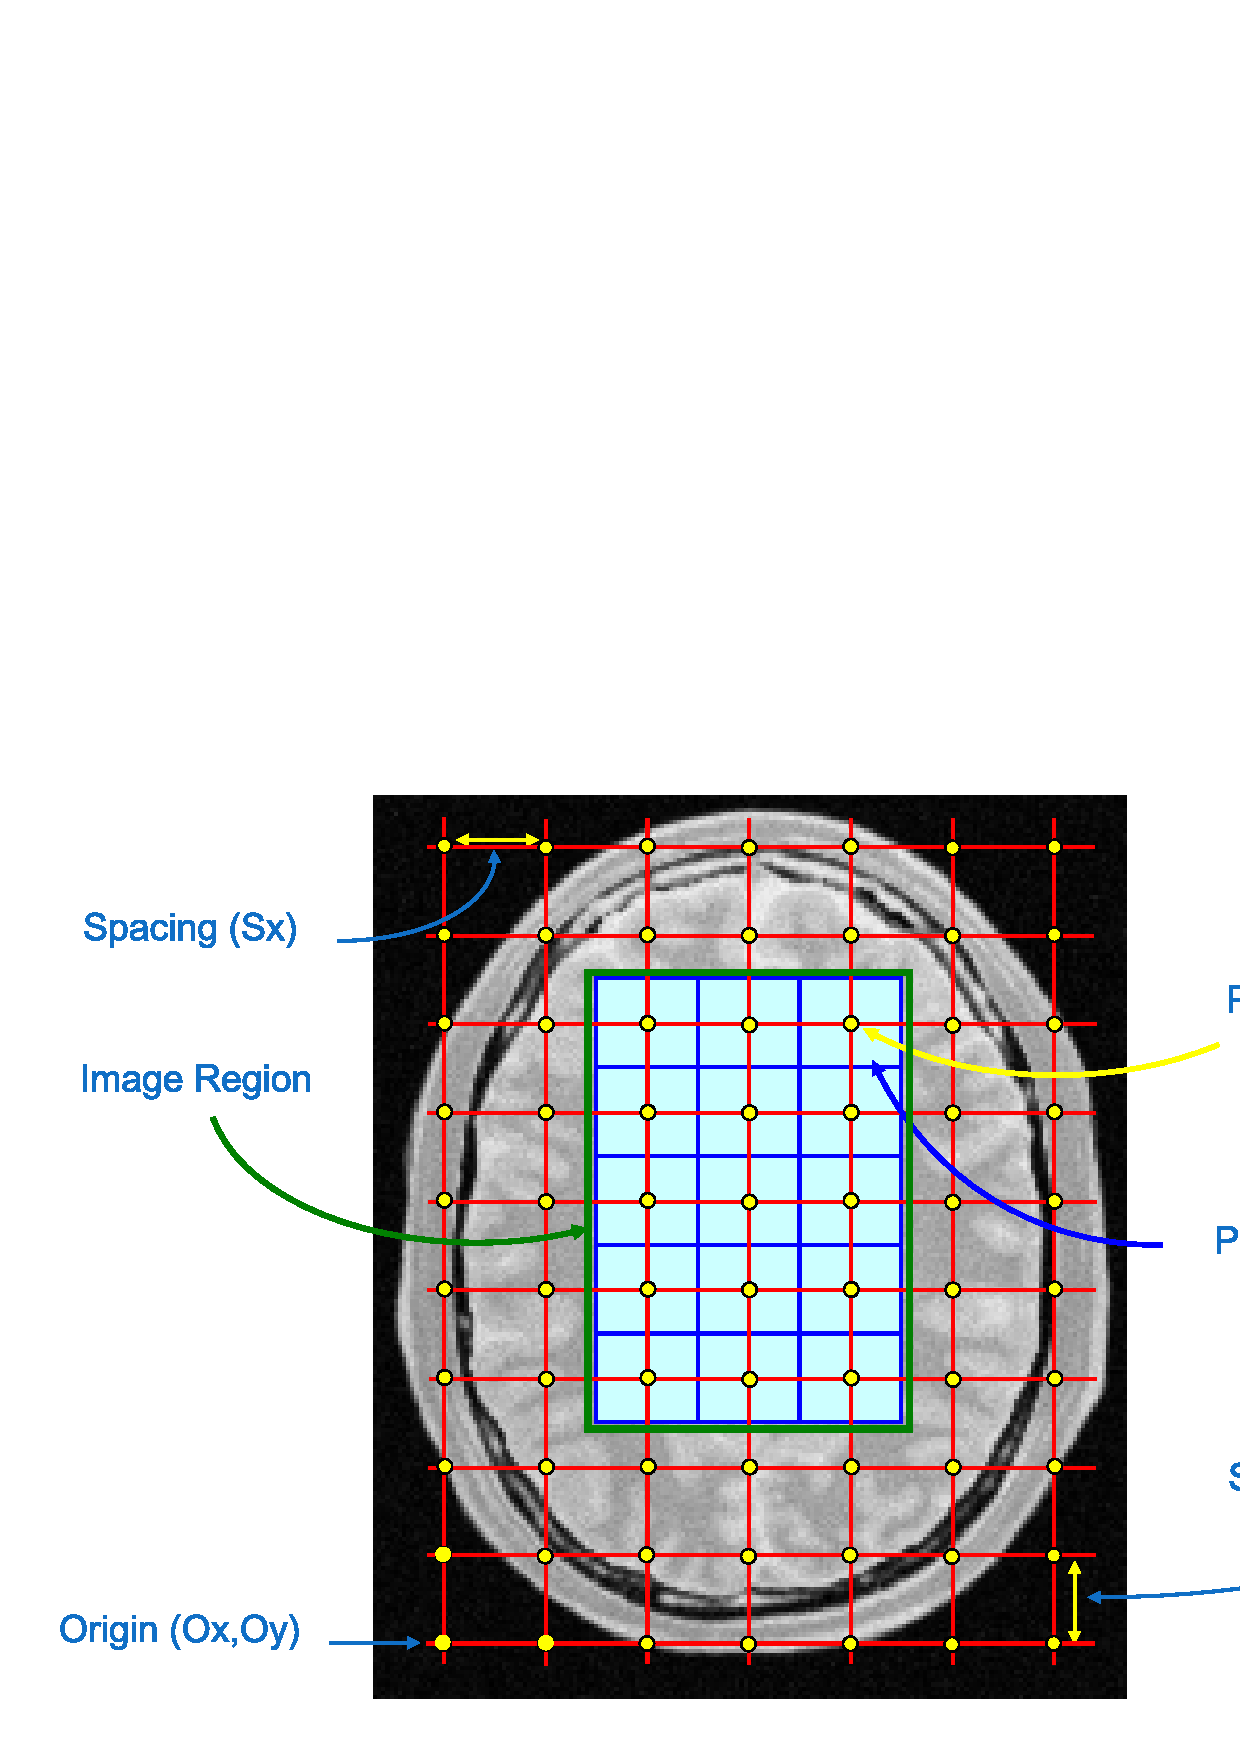
\includegraphics[width=0.8\textwidth]{../Art/Resampling06ImageRegion1.pdf}
\end{frame}

\begin{frame}
  \frametitle{Image Region: Size}
  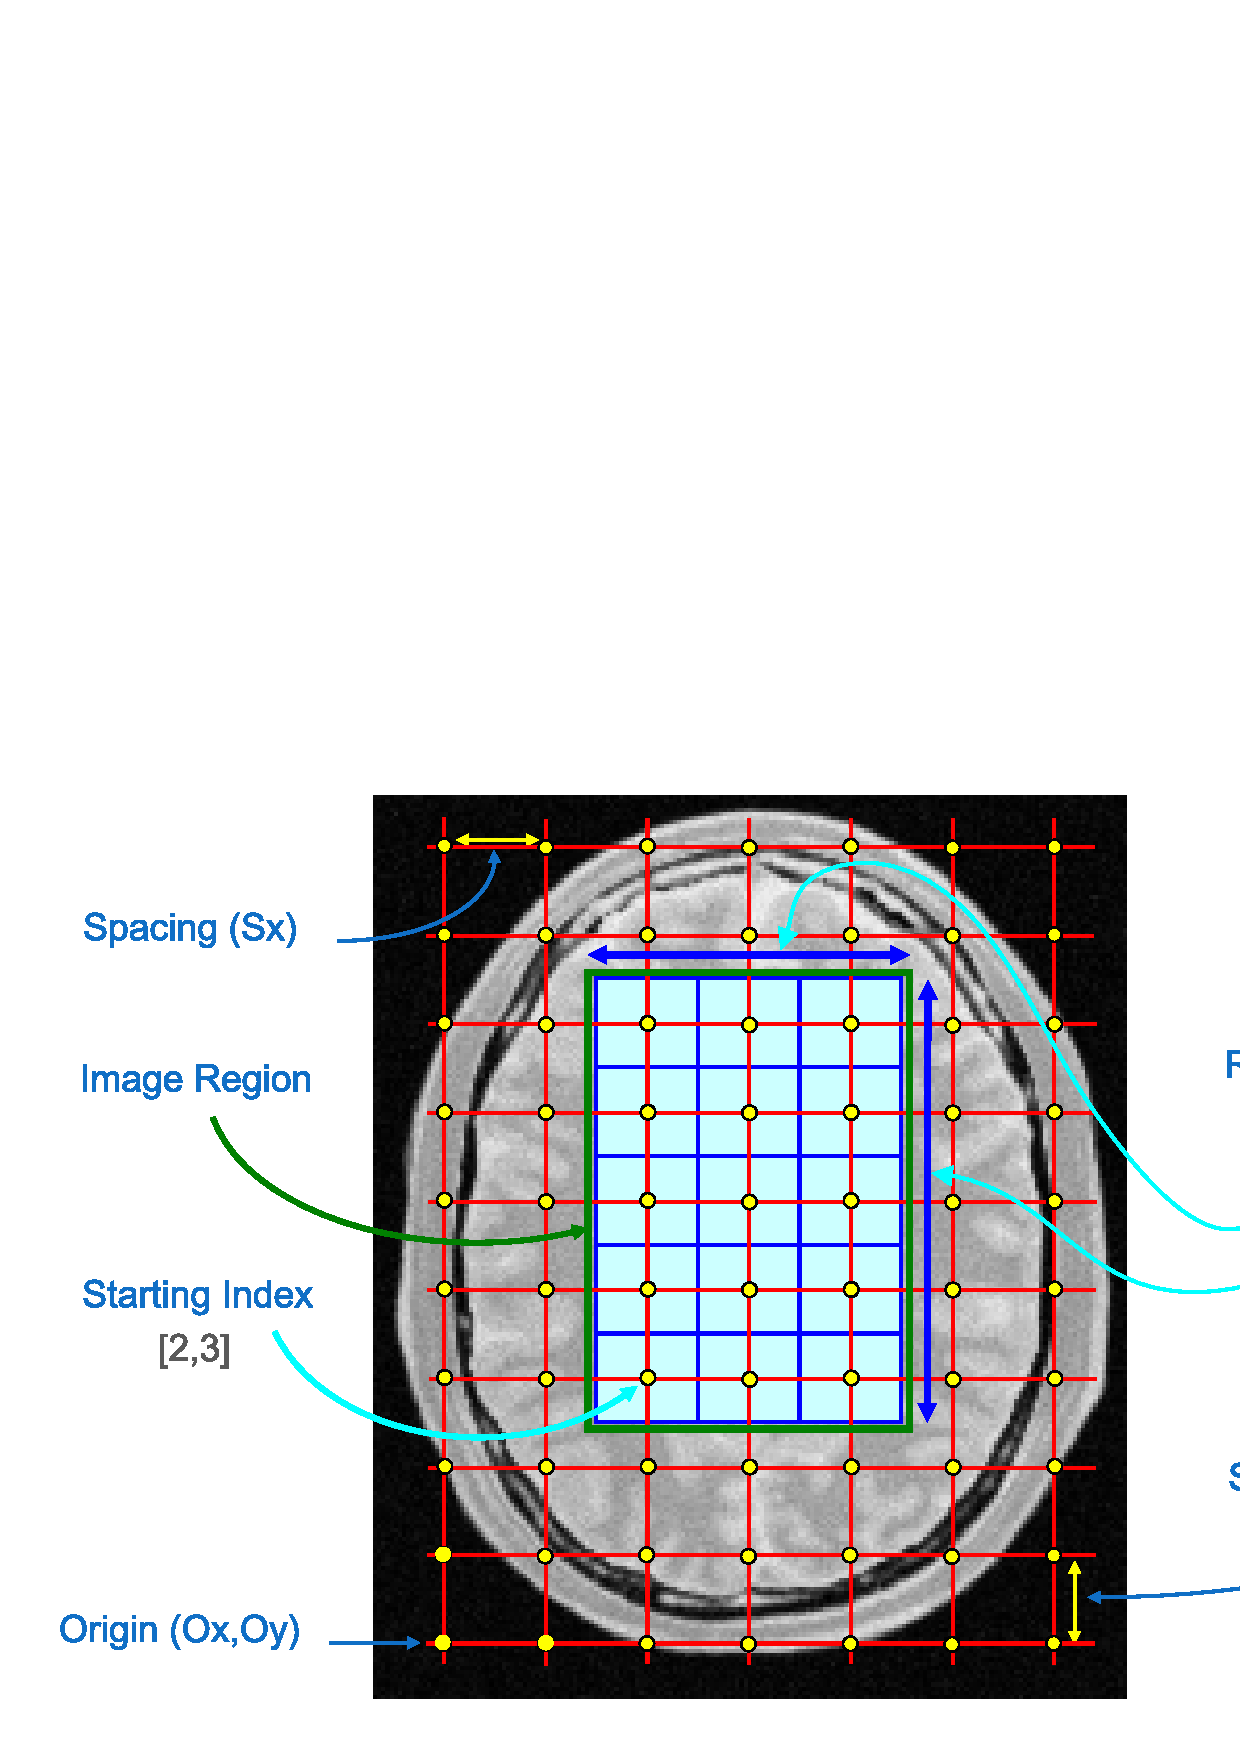
\includegraphics[width=0.8\textwidth]{../Art/Resampling07ImageRegion2.pdf}
\end{frame}

\begin{frame}
  \frametitle{Image Region: Starting Index}
  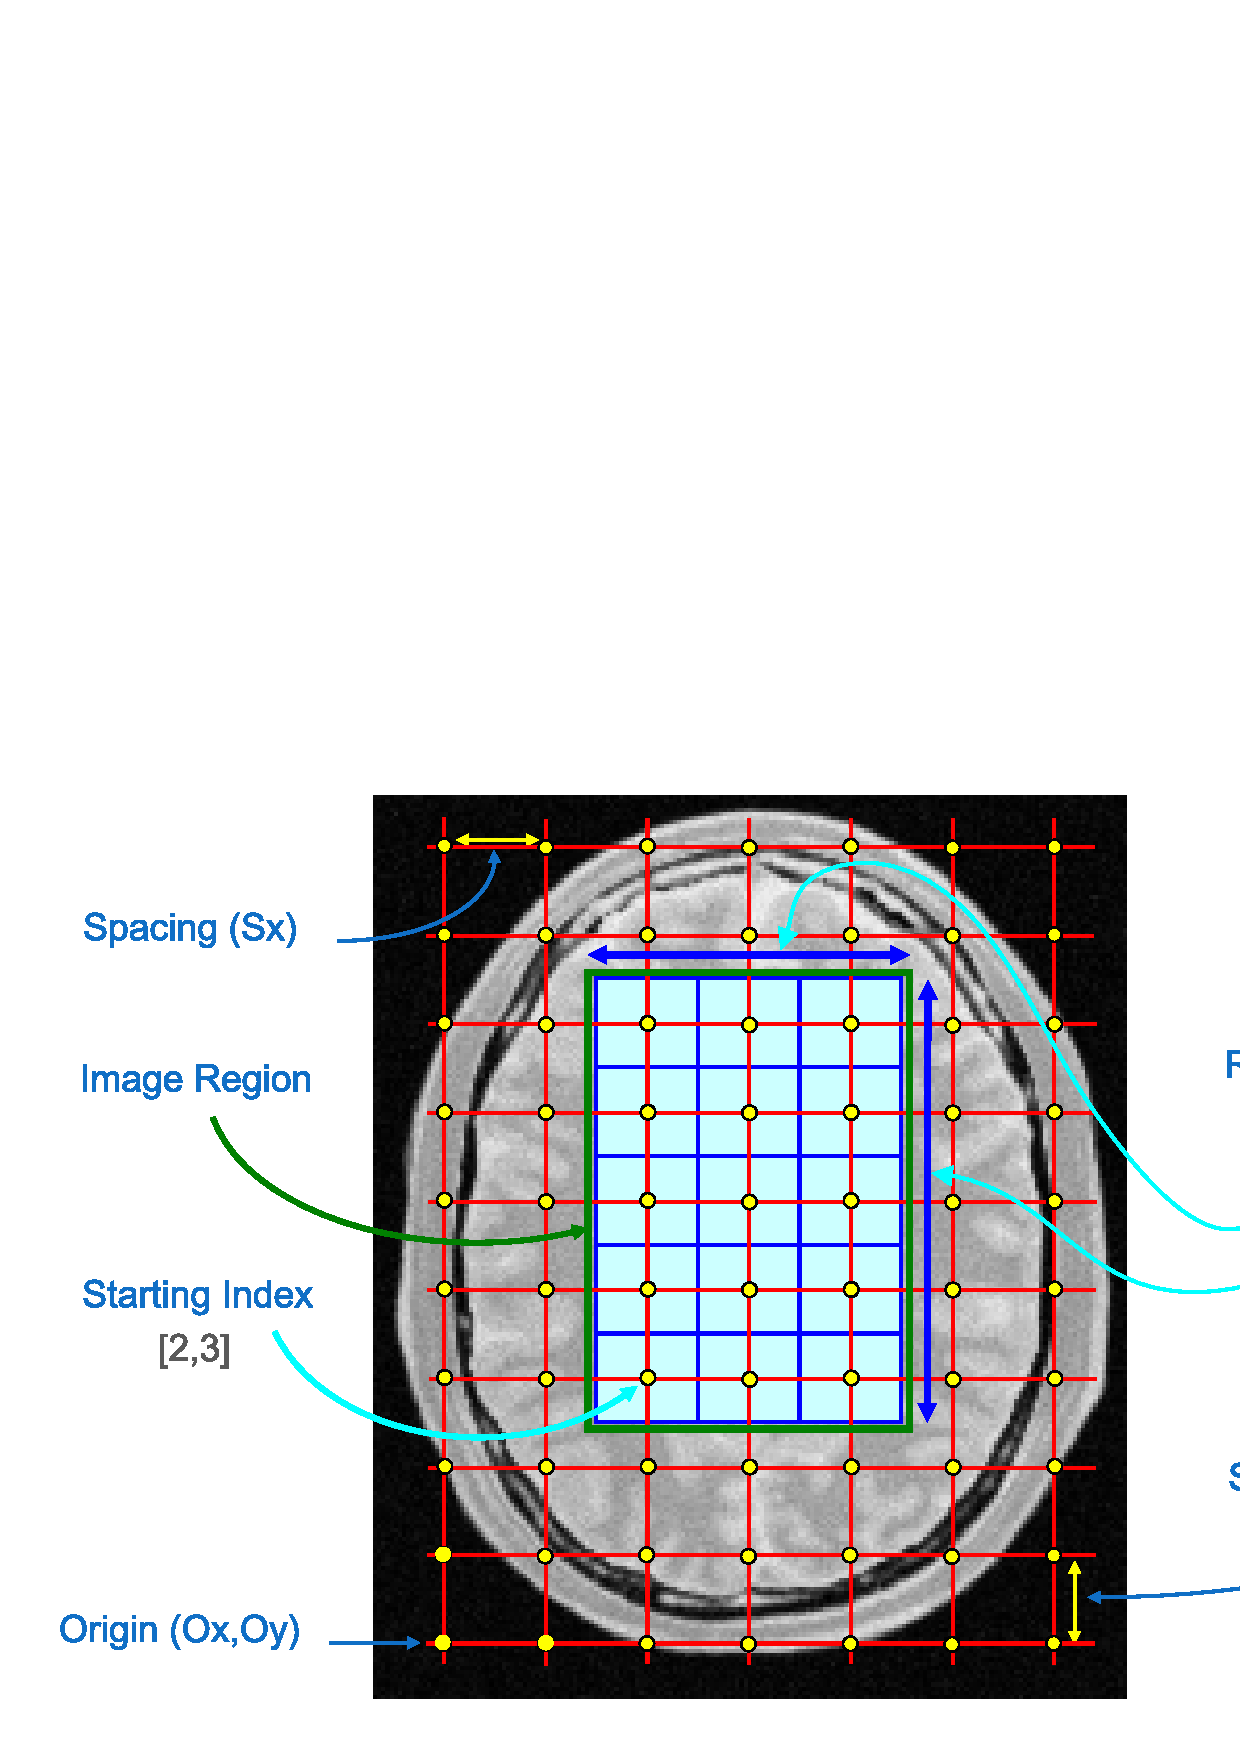
\includegraphics[width=0.8\textwidth]{../Art/Resampling08ImageRegion3.pdf}
\end{frame}

\begin{frame}
  \frametitle{Sub-sampling by Half}
  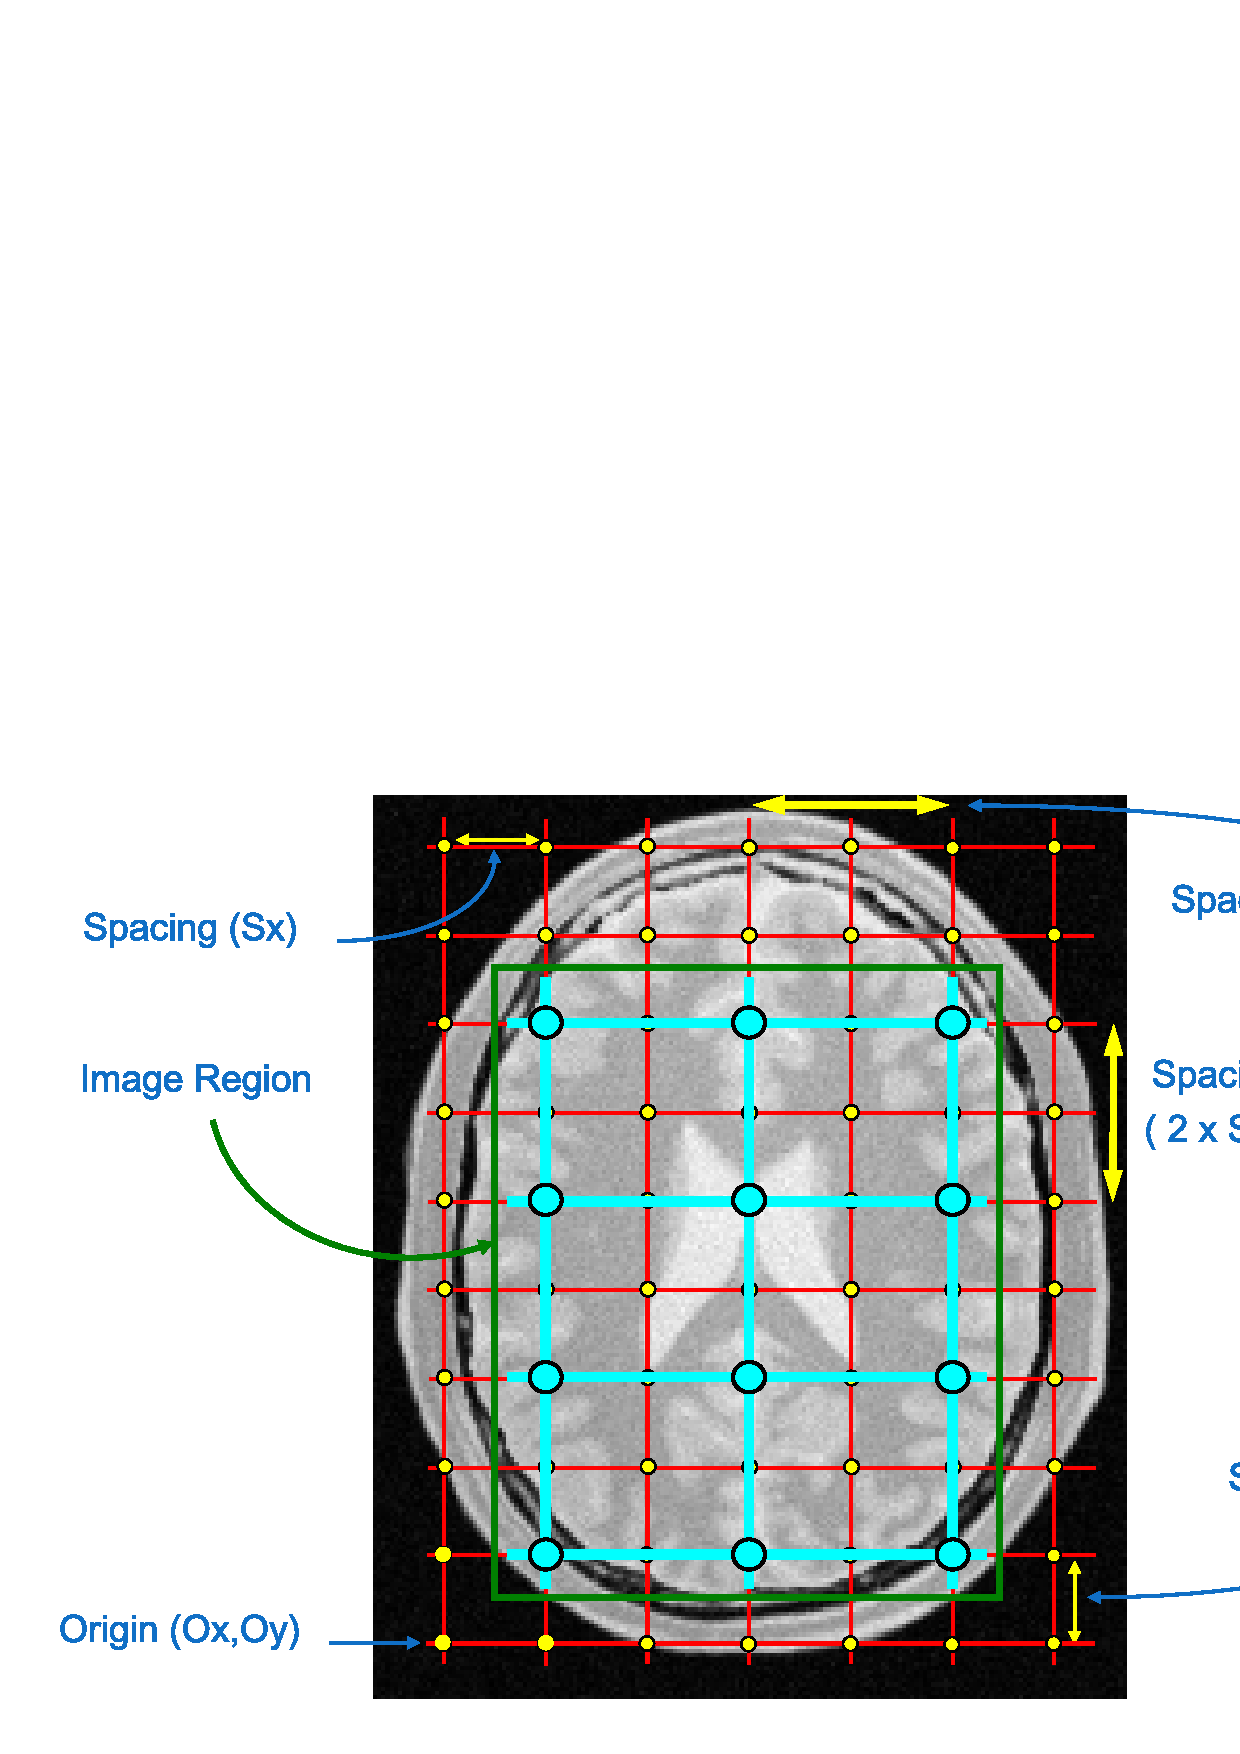
\includegraphics[width=0.8\textwidth]{../Art/Resampling09SubSamplingByHalf1.pdf}
\end{frame}

\begin{frame}
  \frametitle{Sub-sampling by Half}
  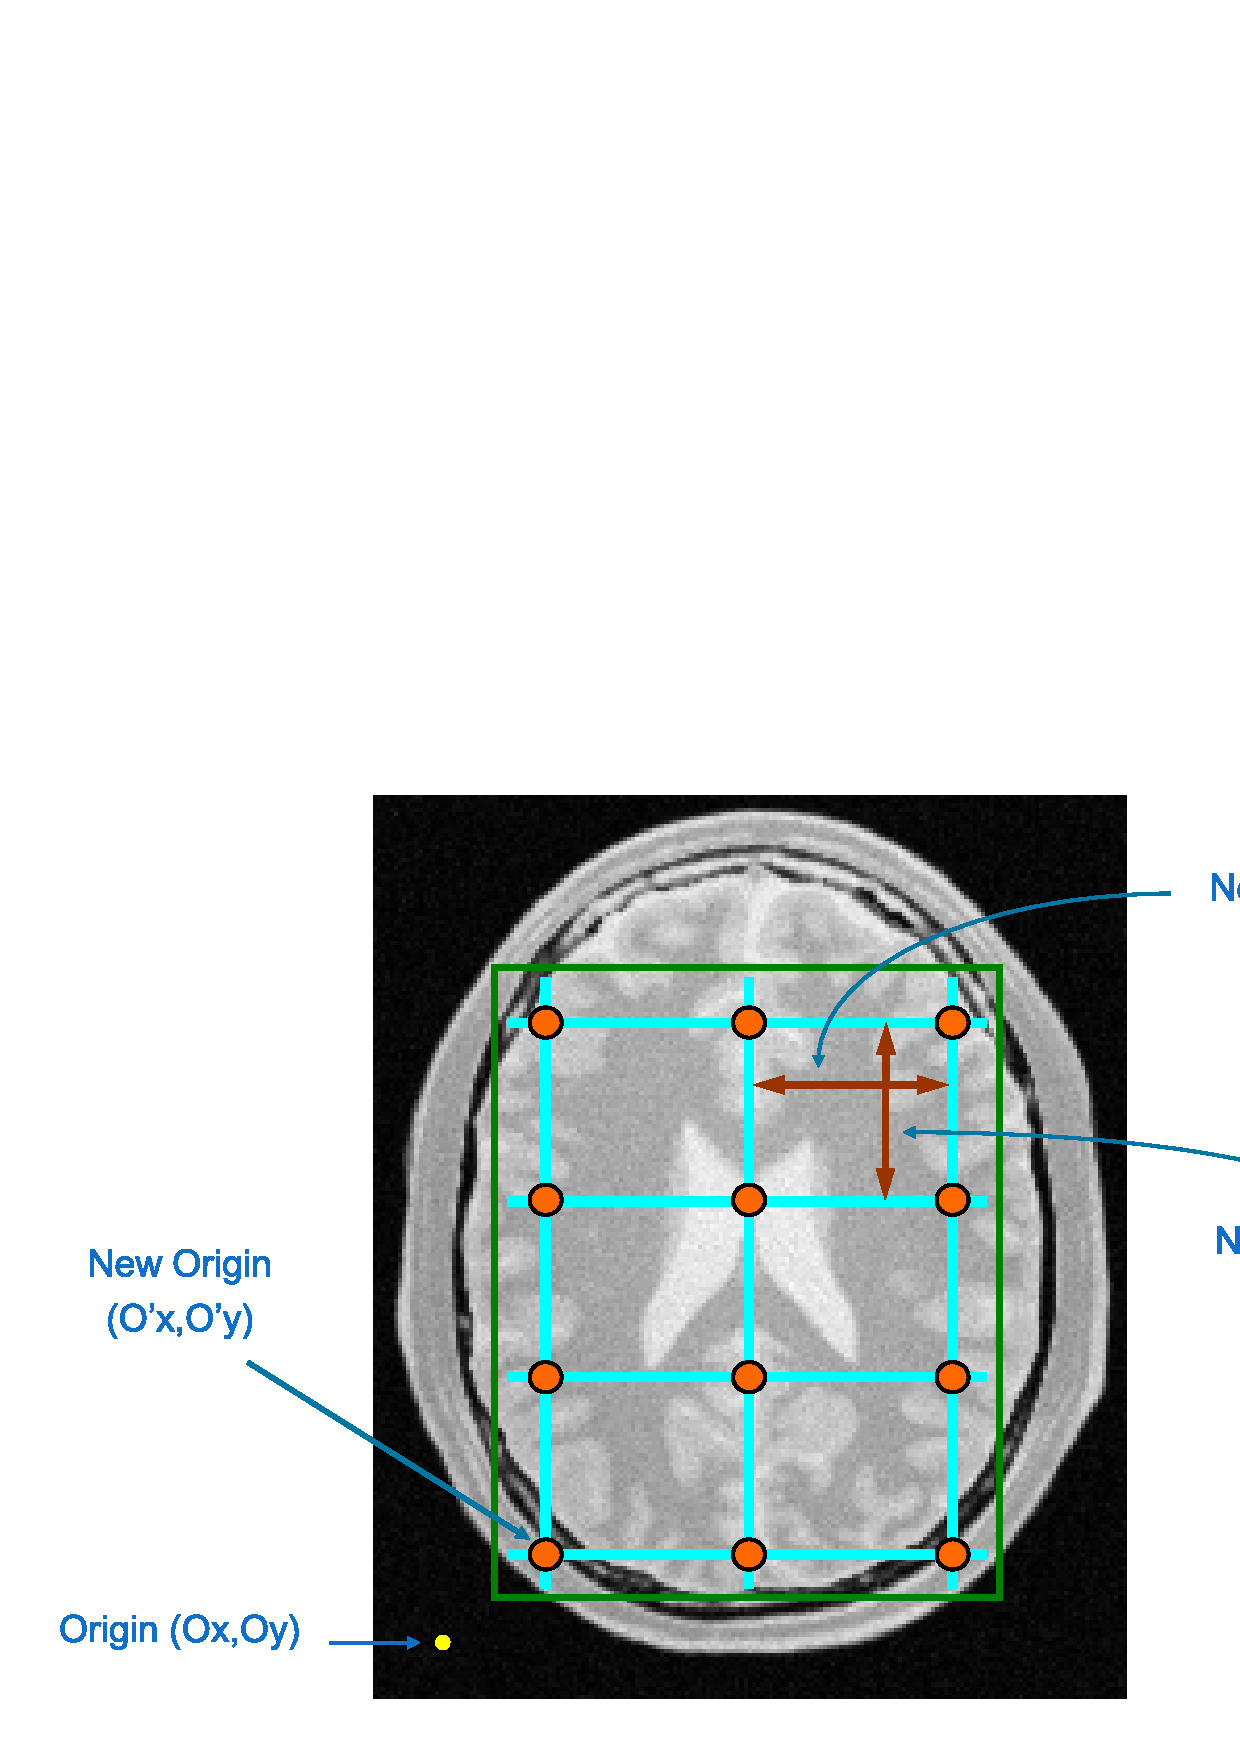
\includegraphics[width=0.8\textwidth]{../Art/Resampling10SubSamplingByHalf2.pdf}
\end{frame}

\begin{frame}
  \frametitle{Super-sampling by Double}
  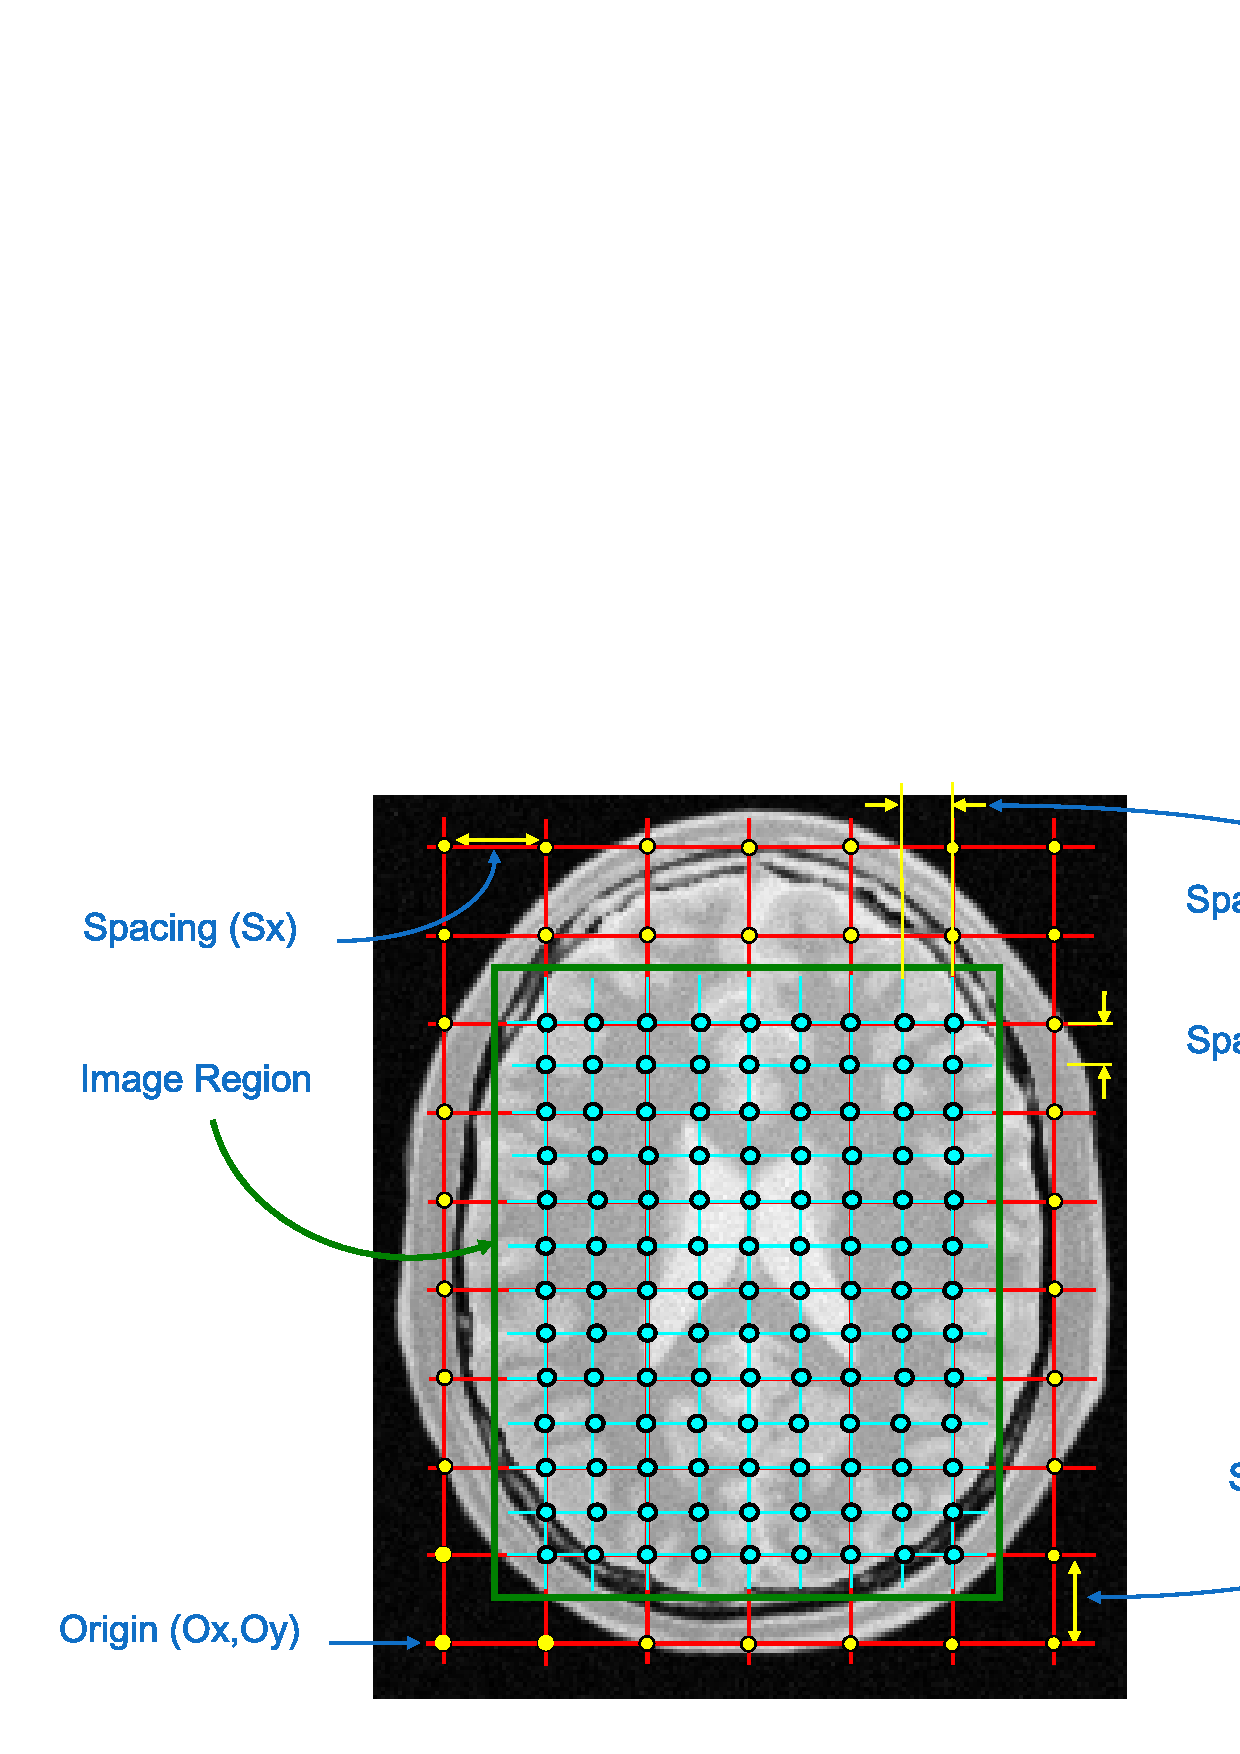
\includegraphics[width=0.8\textwidth]{../Art/Resampling11SuperSamplingByDouble1.pdf}
\end{frame}

\begin{frame}
  \frametitle{Super-sampling by Double}
  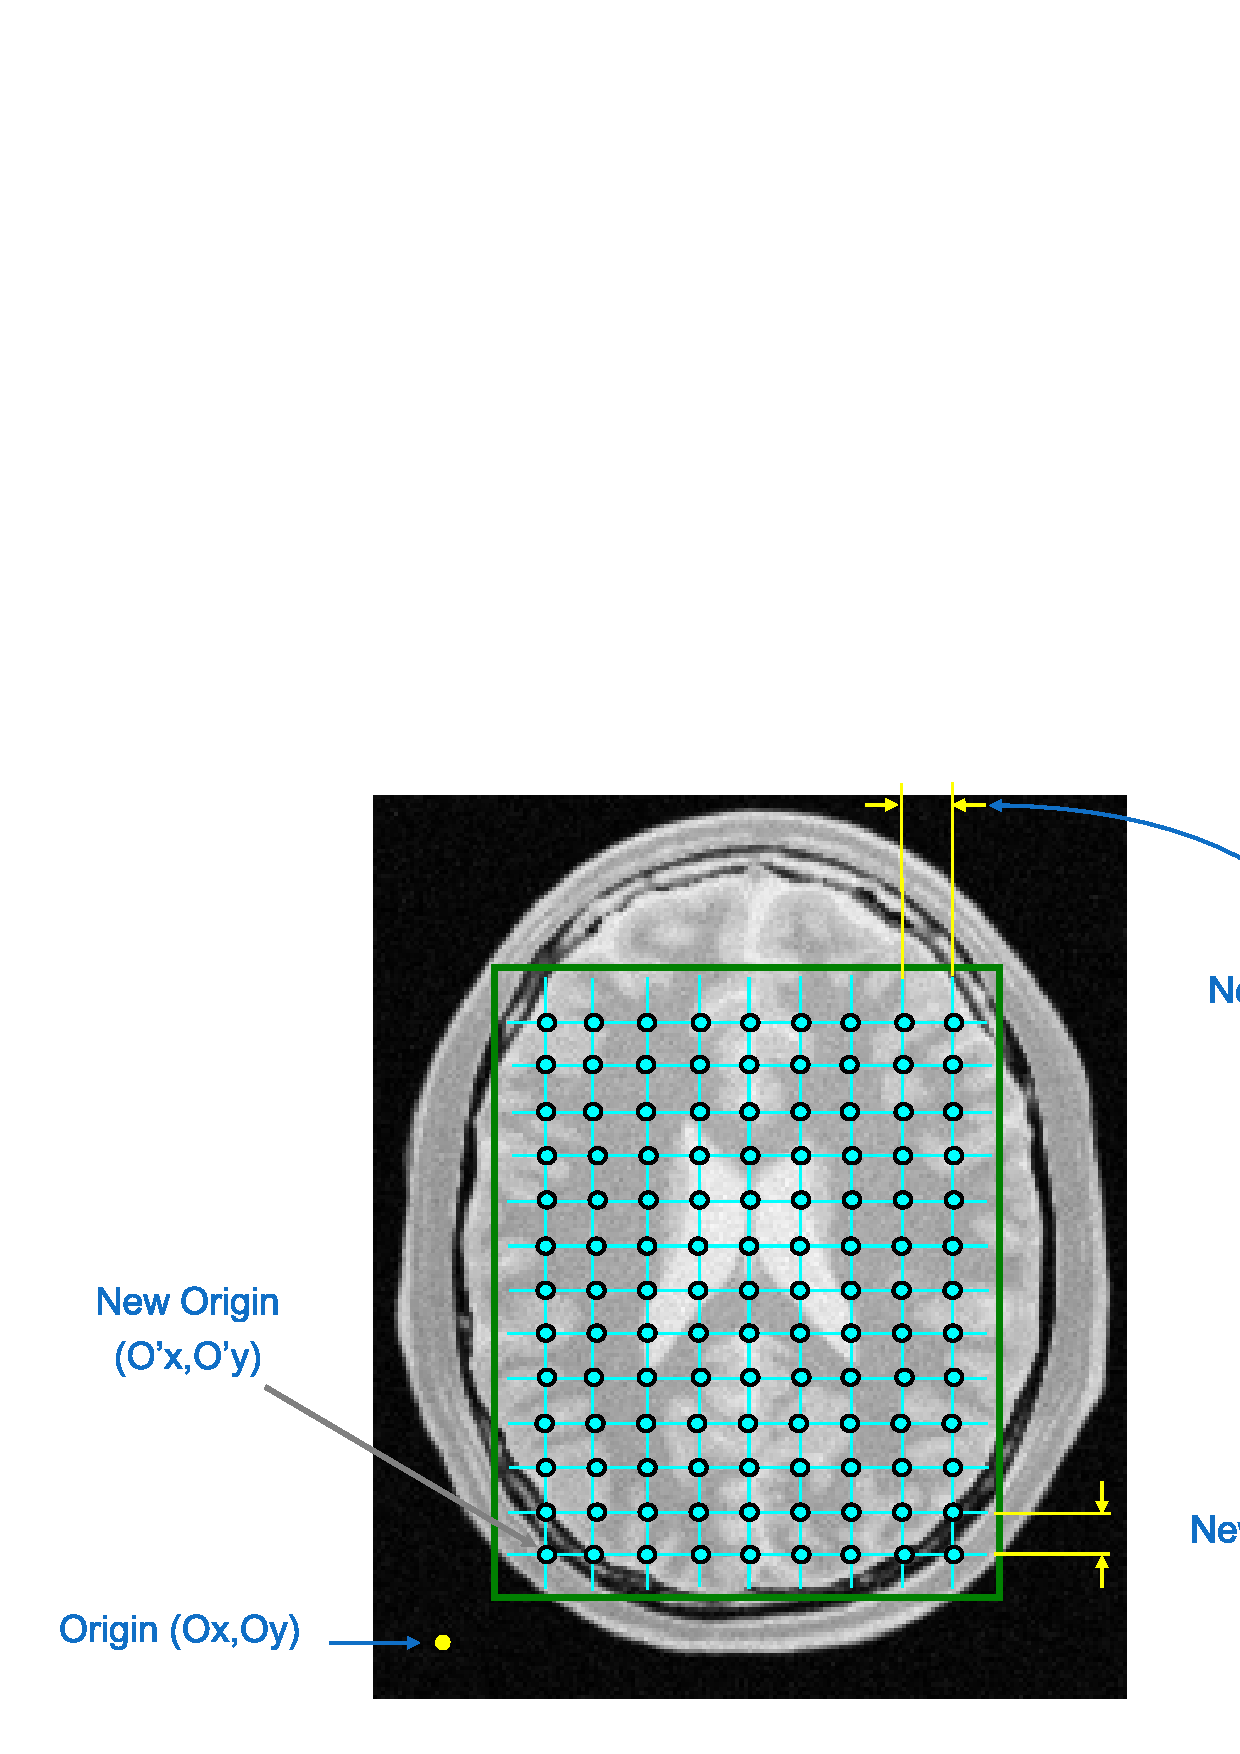
\includegraphics[width=0.8\textwidth]{../Art/Resampling12SuperSamplingByDouble2.pdf}
\end{frame}

\begin{frame}
  \frametitle{Resampling In ITK}
  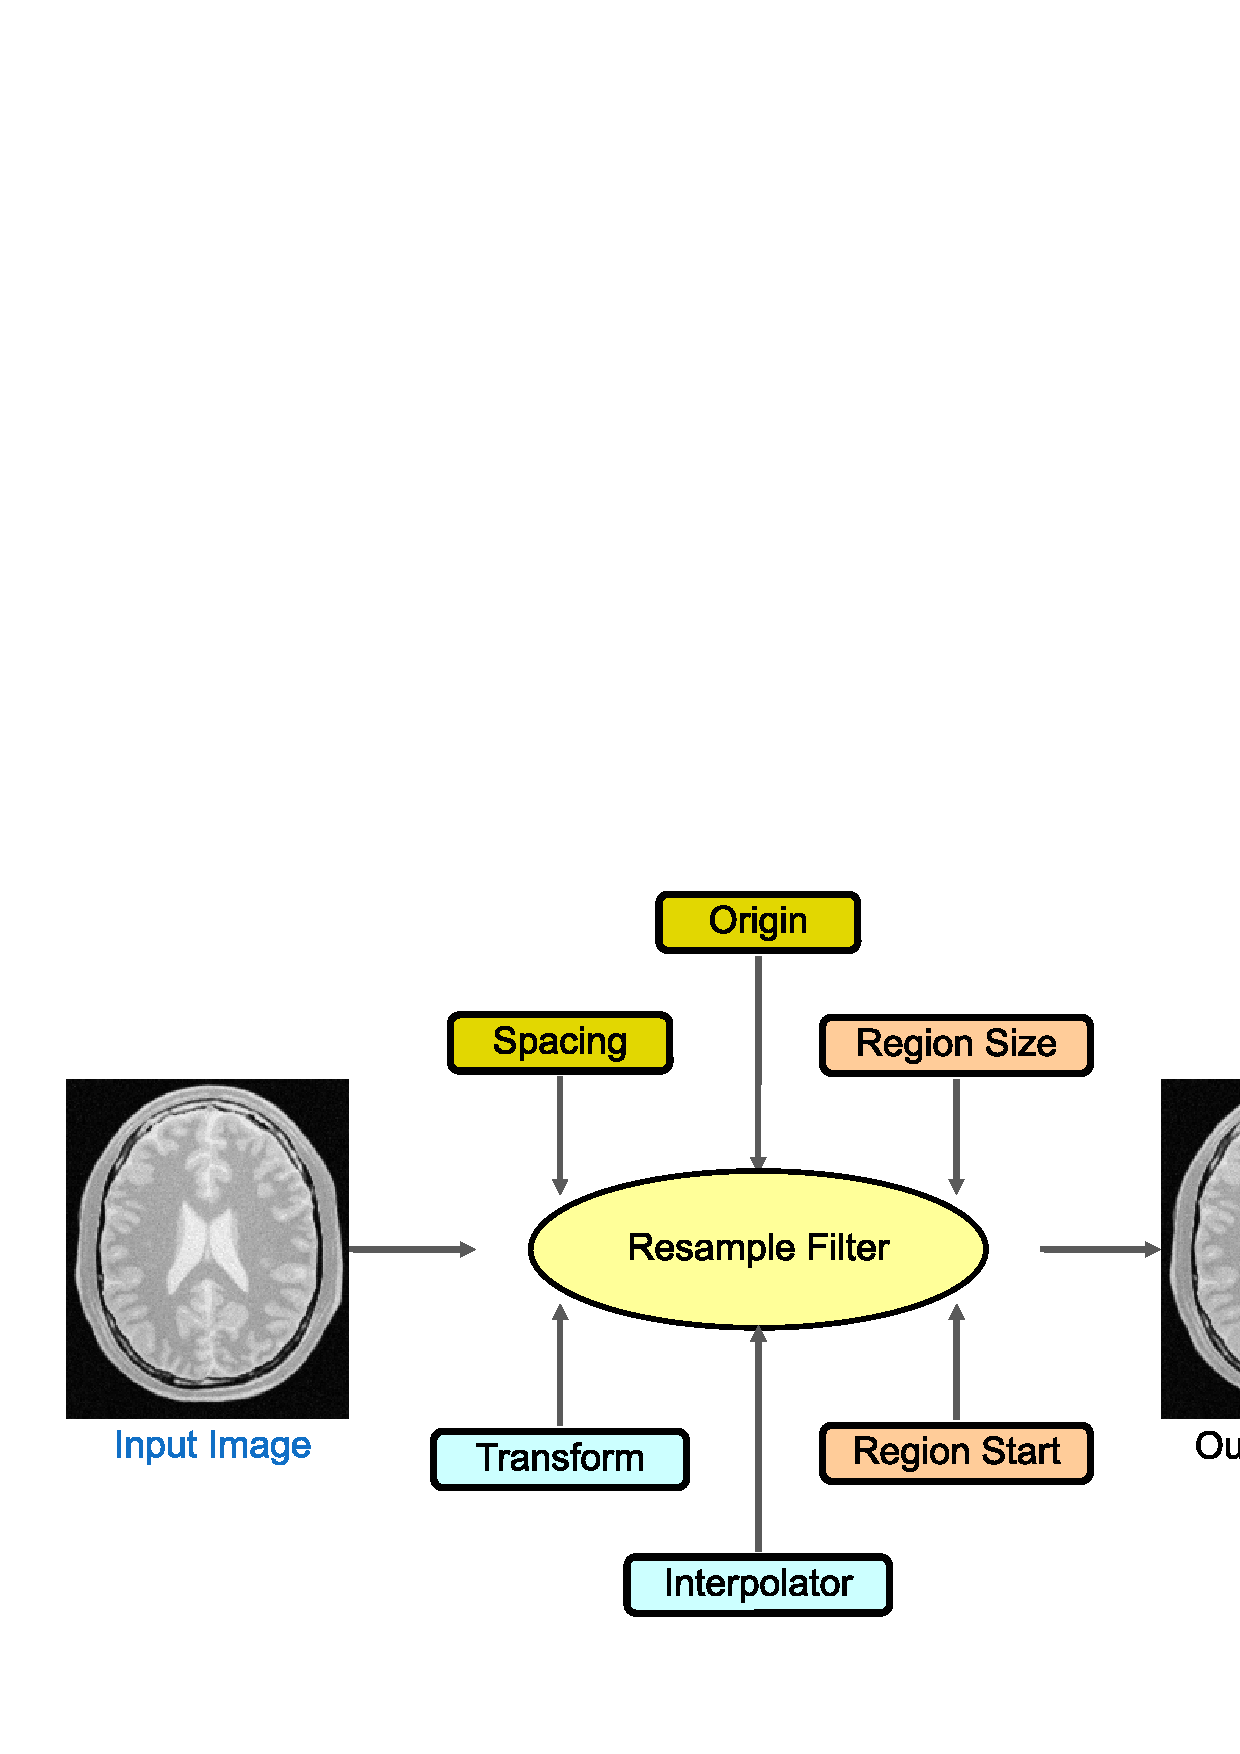
\includegraphics[width=0.8\textwidth]{../Art/Resampling13ResamplingInITK.pdf}
\end{frame}

\begin{frame}
  \frametitle{Coordinate System Conversions}
  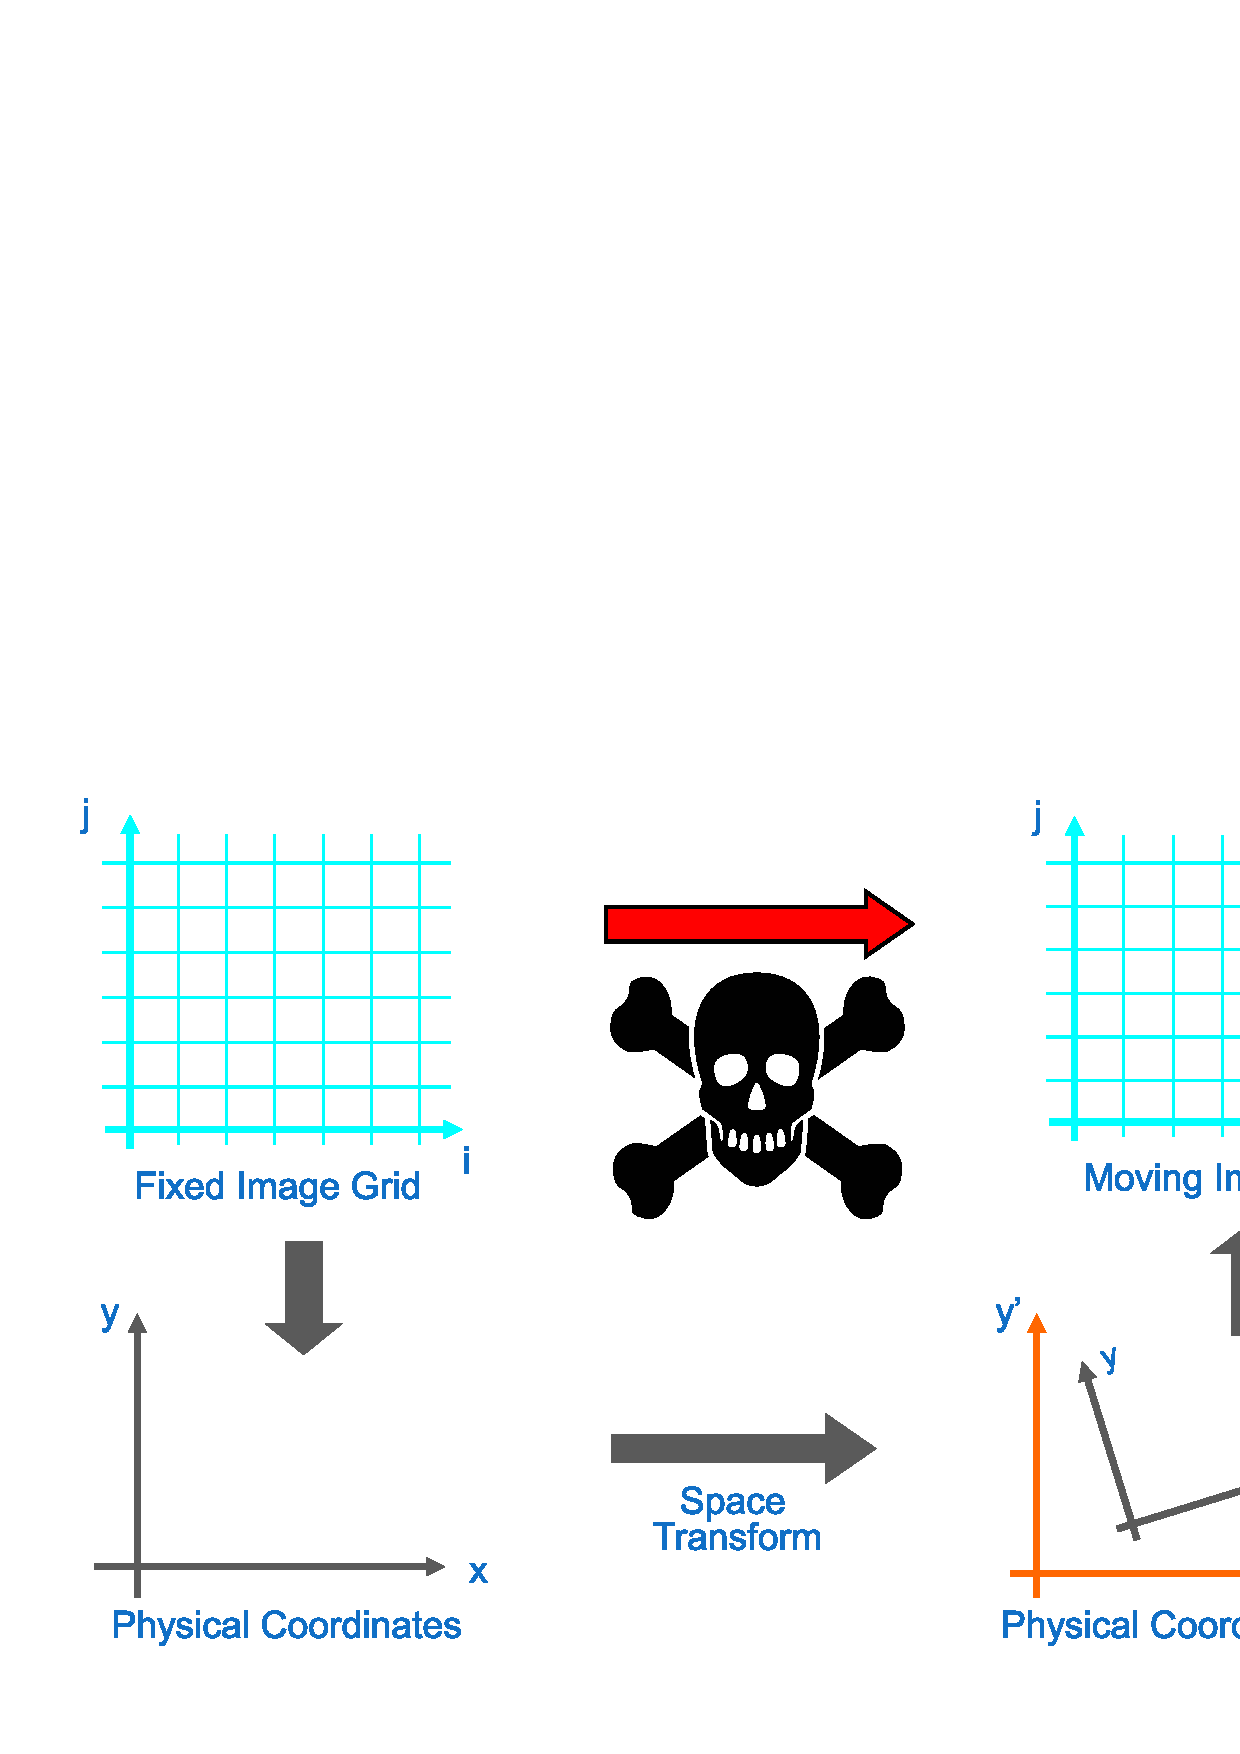
\includegraphics[width=0.8\textwidth]{../Art/Resampling14CoordinateSystemConversions.pdf}
\end{frame}

\subsubsection{Registration}

 \centeredlargetext{white}{black}{
ITK v3 framework
\vskip20pt
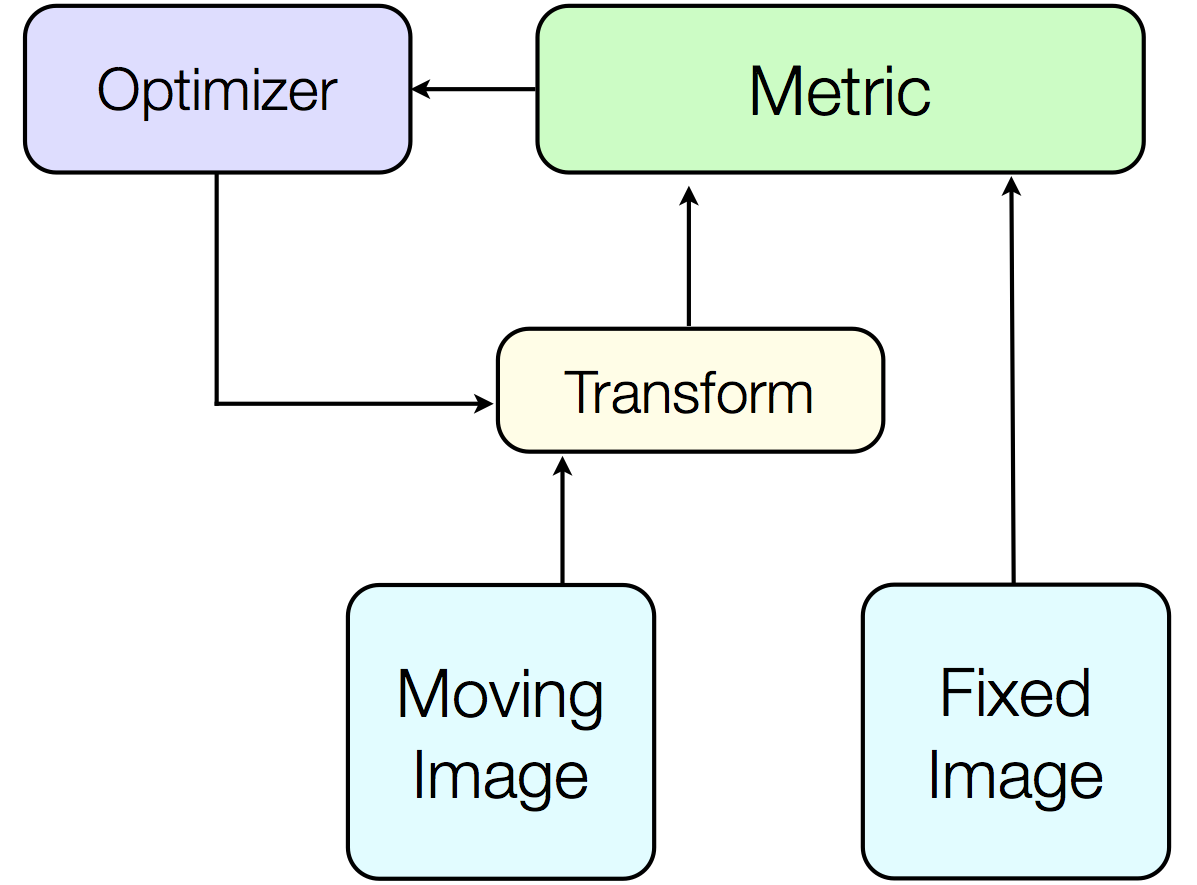
\includegraphics[height=2.2in]{../Art/itkv3reg}
 }

 \centeredlargetext{white}{black}{
ITK v4 framework
\vskip20pt
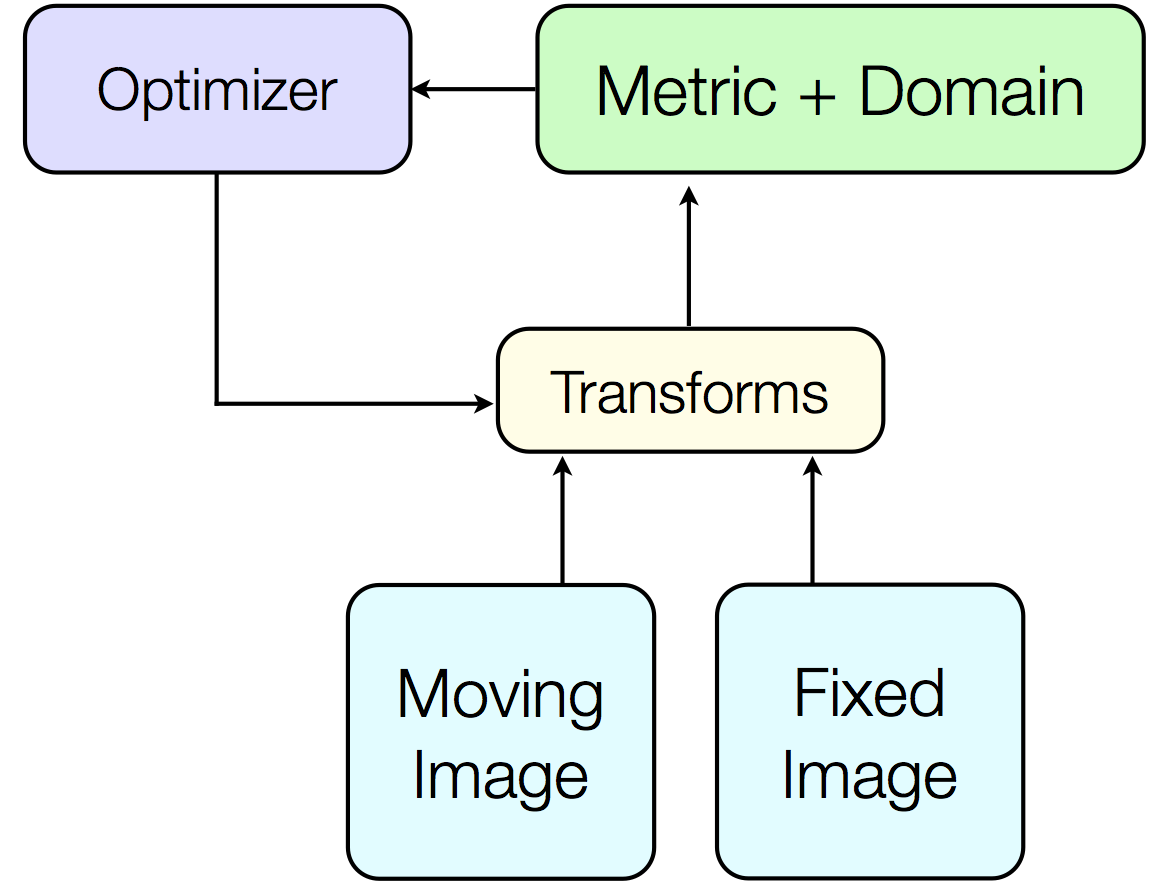
\includegraphics[height=2.2in]{../Art/itkv4reg}
 }

\begin{frame}
\frametitle{Composite transformations}
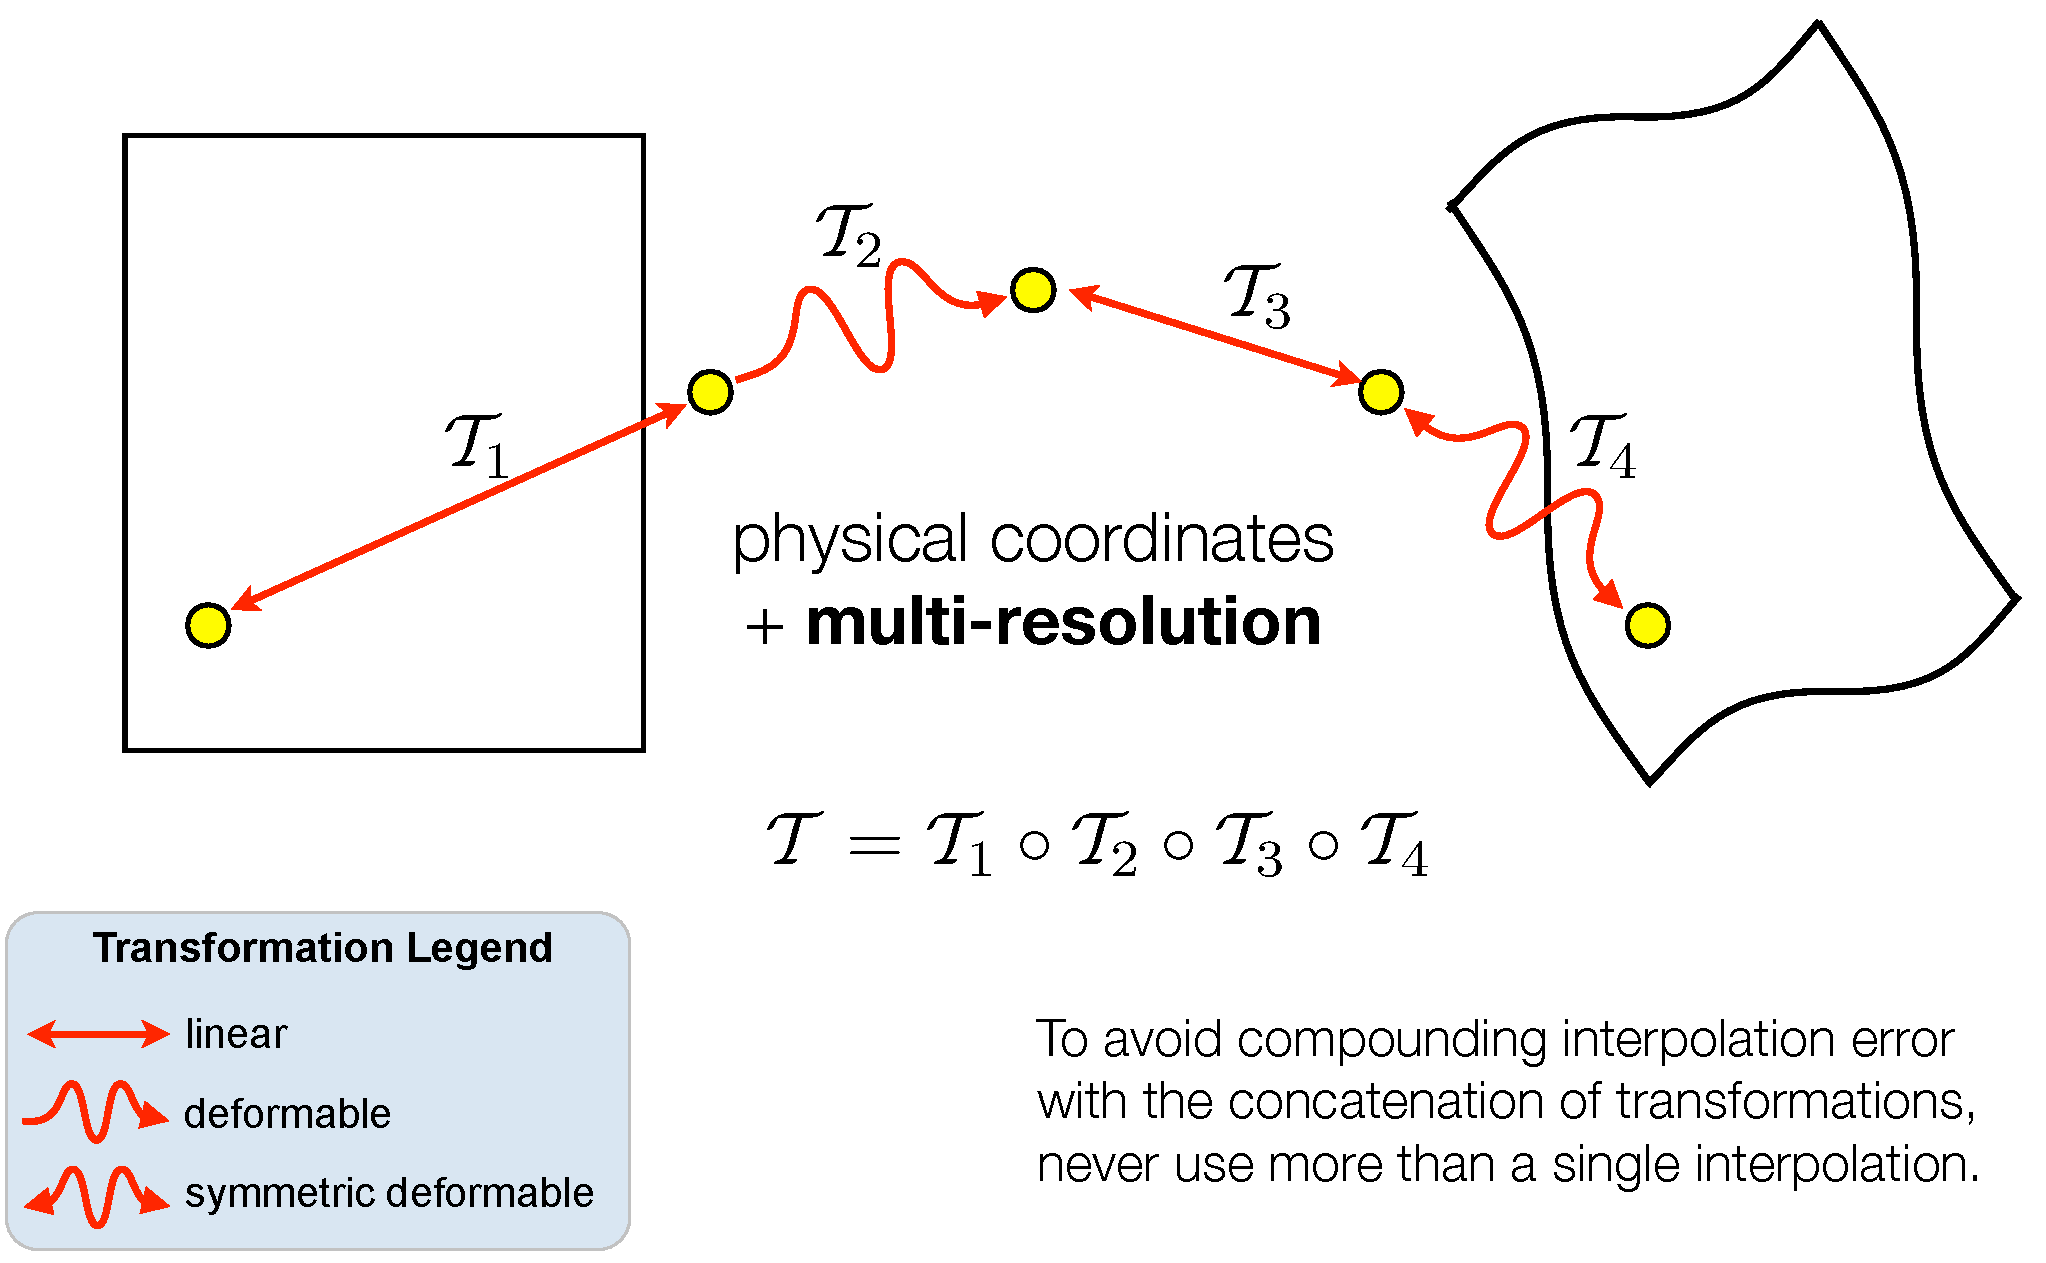
\includegraphics[height=2.5in]{../Art/composite}
\end{frame}

\subsection{Exercise}

 \centeredlargetext{white}{black}{
\centering Example Registration
}

\begin{frame}[fragile]
\frametitle{Example: Perform a simple registration}
\begin{verbatim}
leafpad ~/src/ITKv4-TheNextGeneration-Tutorial/\
Exercises/Registration/RegistrationExercises.cxx &

ImageViewer ~/data/BrainProtonDensitySliceBorder20.png &
ImageViewer ~/data/BrainProtonDensitySliceR10X13Y17.png &
\end{verbatim}
\end{frame}

\begin{frame}[fragile]
\frametitle{Example: Perform a simple registration}
\begin{verbatim}
./bin/RegistrationExercises ~/data/BrainProtonDensitySliceBorder20.png \
  ~/data/BrainProtonDensitySliceR10X13Y17.png \
  ./Registered.png \
  3000

ImageViewer ./Registered.png &
\end{verbatim}
\end{frame}

\begin{frame}[fragile]
\frametitle{Exercise: Do not scale the optimizer parameters}
  \begin{itemize}
    \item In \texttt{RegistrationExercises.cxx}, \textbf{line 163}, turn off
      automatic optimizer paramer scaling.
    \item What happens and why?
  \end{itemize}
\end{frame}
